% =====================================================================
% TVT submission freeze, manuscript version V6 Final (2026-08-27).
% V6 preserves the V5.5 factual record while centering one evidence chain:
% condition-dependent ranking, independent severe-regime transport boundary,
% representation diagnosis, and low-cost received-I/Q repair.
% Self-contained: this manuscript relies on no
% supplementary document for its claims; it points to the optional standalone
% supplement for audit-level tables (covariate ladder, selector, convergence,
% sidecar structure, control breakdowns).
% =====================================================================
\documentclass[letterpaper,journal]{IEEEtran}

\usepackage[T1]{fontenc}
\usepackage{amsmath,amssymb}
\usepackage{booktabs}
\usepackage{graphicx}
\usepackage{xcolor}
\usepackage{cite}
\usepackage[hidelinks]{hyperref}

\newif\ifinternalreview
\internalreviewtrue

% Safe internal-review placeholder for the complete public-table contract.
% A release writer must replace every value and add EligibleLockedResults.
\newcommand{\ResultSource}{No eligible locked run}
\newcommand{\PrimaryReference}{--}
\newcommand{\VIMDLatencyDevice}{--}
\newcommand{\HeadlineHardAZeroAccuracy}{--}
\newcommand{\HeadlineHardAZeroMacroFOne}{--}
\newcommand{\HeadlineHardAZeroWorstRecall}{--}
\newcommand{\HeadlineHardAZeroNLL}{--}
\newcommand{\HeadlineHardAZeroECE}{--}
\newcommand{\HeadlineHardMCLDNNAccuracy}{--}
\newcommand{\HeadlineHardMCLDNNMacroFOne}{--}
\newcommand{\HeadlineHardMCLDNNWorstRecall}{--}
\newcommand{\HeadlineHardMCLDNNNLL}{--}
\newcommand{\HeadlineHardMCLDNNECE}{--}
\newcommand{\HeadlineHardIQFormerAccuracy}{--}
\newcommand{\HeadlineHardIQFormerMacroFOne}{--}
\newcommand{\HeadlineHardIQFormerWorstRecall}{--}
\newcommand{\HeadlineHardIQFormerNLL}{--}
\newcommand{\HeadlineHardIQFormerECE}{--}
\newcommand{\HeadlineHardCSSLAccuracy}{--}
\newcommand{\HeadlineHardCSSLMacroFOne}{--}
\newcommand{\HeadlineHardCSSLWorstRecall}{--}
\newcommand{\HeadlineHardCSSLNLL}{--}
\newcommand{\HeadlineHardCSSLECE}{--}
\newcommand{\HeadlineHardAFiveAccuracy}{--}
\newcommand{\HeadlineHardAFiveMacroFOne}{--}
\newcommand{\HeadlineHardAFiveWorstRecall}{--}
\newcommand{\HeadlineHardAFiveNLL}{--}
\newcommand{\HeadlineHardAFiveECE}{--}
\newcommand{\HeadlineHardAOneMacroFOne}{--}
\newcommand{\HeadlineHardATwoMacroFOne}{--}
\newcommand{\HeadlineHardAThreePrimeMacroFOne}{--}
\newcommand{\HeadlineHardAThreeMacroFOne}{--}
\newcommand{\HeadlineHardAFourMacroFOne}{--}
\newcommand{\HeadlineHardASixMacroFOne}{--}
\newcommand{\HeadlineHardASevenMacroFOne}{--}
\newcommand{\AblationFullVsBackboneGain}{--}
\newcommand{\AblationFullVsBackboneCILow}{--}
\newcommand{\AblationFullVsBackboneCIHigh}{--}
\newcommand{\AblationMarginVsProportionalGain}{--}
\newcommand{\AblationMarginVsProportionalCILow}{--}
\newcommand{\AblationMarginVsProportionalCIHigh}{--}
\newcommand{\AblationTeacherGain}{--}
\newcommand{\AblationTeacherCILow}{--}
\newcommand{\AblationTeacherCIHigh}{--}
\newcommand{\AblationMultitaskGain}{--}
\newcommand{\AblationMultitaskCILow}{--}
\newcommand{\AblationMultitaskCIHigh}{--}
\newcommand{\AblationExactSourceContrastGain}{--}
\newcommand{\AblationExactSourceContrastCILow}{--}
\newcommand{\AblationExactSourceContrastCIHigh}{--}
\newcommand{\AblationFullVsSingleGain}{--}
\newcommand{\AblationFullVsSingleCILow}{--}
\newcommand{\AblationFullVsSingleCIHigh}{--}
\newcommand{\AblationFullVsDualGain}{--}
\newcommand{\AblationFullVsDualCILow}{--}
\newcommand{\AblationFullVsDualCIHigh}{--}
\newcommand{\AblationBypassGain}{--}
\newcommand{\AblationBypassCILow}{--}
\newcommand{\AblationBypassCIHigh}{--}
\newcommand{\RegimeHardAZero}{--}
\newcommand{\RegimeHardAFive}{--}
\newcommand{\RegimeHardGain}{--}
\newcommand{\RegimeHardCILow}{--}
\newcommand{\RegimeHardCIHigh}{--}
\newcommand{\RegimeUnseenJammerAZero}{--}
\newcommand{\RegimeUnseenJammerAFive}{--}
\newcommand{\RegimeUnseenJammerGain}{--}
\newcommand{\RegimeUnseenJammerCILow}{--}
\newcommand{\RegimeUnseenJammerCIHigh}{--}
\newcommand{\RegimeUnseenSpeedAZero}{--}
\newcommand{\RegimeUnseenSpeedAFive}{--}
\newcommand{\RegimeUnseenSpeedGain}{--}
\newcommand{\RegimeUnseenSpeedCILow}{--}
\newcommand{\RegimeUnseenSpeedCIHigh}{--}
\newcommand{\RegimeHeldoutChannelAZero}{--}
\newcommand{\RegimeHeldoutChannelAFive}{--}
\newcommand{\RegimeHeldoutChannelGain}{--}
\newcommand{\RegimeHeldoutChannelCILow}{--}
\newcommand{\RegimeHeldoutChannelCIHigh}{--}
\newcommand{\RegimeCombinedOODAZero}{--}
\newcommand{\RegimeCombinedOODAFive}{--}
\newcommand{\RegimeCombinedOODGain}{--}
\newcommand{\RegimeCombinedOODCILow}{--}
\newcommand{\RegimeCombinedOODCIHigh}{--}
\newcommand{\RegimeCleanACDCSSL}{--}
\newcommand{\RegimeCleanACDAFive}{--}
\newcommand{\RegimeCleanACDGain}{--}
\newcommand{\RegimeCleanACDCILow}{--}
\newcommand{\RegimeCleanACDCIHigh}{--}
\newcommand{\RegimeCleanBECSSL}{--}
\newcommand{\RegimeCleanBEAFive}{--}
\newcommand{\RegimeCleanBEGain}{--}
\newcommand{\RegimeCleanBECILow}{--}
\newcommand{\RegimeCleanBECIHigh}{--}
\newcommand{\RegimeADCTenAZero}{--}
\newcommand{\RegimeADCTenAFive}{--}
\newcommand{\RegimeADCTenGain}{--}
\newcommand{\RegimeADCTenCILow}{--}
\newcommand{\RegimeADCTenCIHigh}{--}
\newcommand{\RegimeADCTwelveAZero}{--}
\newcommand{\RegimeADCTwelveAFive}{--}
\newcommand{\RegimeADCTwelveGain}{--}
\newcommand{\RegimeADCTwelveCILow}{--}
\newcommand{\RegimeADCTwelveCIHigh}{--}
\newcommand{\RegimeEmitterSyncAZero}{--}
\newcommand{\RegimeEmitterSyncAFive}{--}
\newcommand{\RegimeEmitterSyncGain}{--}
\newcommand{\RegimeEmitterSyncCILow}{--}
\newcommand{\RegimeEmitterSyncCIHigh}{--}
\newcommand{\MechanismMaskJS}{--}
\newcommand{\MechanismThirdRouteWeightedCorrelation}{--}
\newcommand{\MechanismTargetTransferRatio}{--}
\newcommand{\MechanismTargetAmplificationShare}{--}
\newcommand{\MechanismJammerLeakage}{--}
\newcommand{\MechanismThirdRouteSpearman}{--}
\newcommand{\MechanismThirdRoutePermutationP}{--}
\newcommand{\OracleSpectralRatioGain}{--}
\newcommand{\MechanismOccupancyGainSpearman}{--}
\newcommand{\MechanismOccupancyGainPermutationP}{--}
\newcommand{\VIMDParameters}{--}
\newcommand{\VIMDLatencyPFifty}{--}
\newcommand{\VIMDLatencyPNinetyFive}{--}


\ifinternalreview\else
  \ifdefined\EligibleLockedResults\else
    \PackageError{VIMD-Net evidence lock}
      {Public build requires \string\EligibleLockedResults\space from an eligible locked run}
      {Regenerate results_auto.tex from the frozen evidence pipeline before submission.}
  \fi
\fi

% All empirical values are generated from artifact-backed CSV/JSON files.
% Generated by paper_data_layer/build_paper_numbers.py -- do not edit by hand.
% Every value carries an evidence class; see outputs/paper_numbers.json.

\newcommand{\AbsAFiveClean}{0.5005}% sealed
\newcommand{\AbsAFiveHard}{0.4406}% sealed
\newcommand{\AbsAFiveId}{0.5654}% sealed
\newcommand{\AbsAZeroClean}{0.4705}% sealed
\newcommand{\AbsAZeroHard}{0.3949}% sealed
\newcommand{\AbsAZeroId}{0.5102}% sealed
\newcommand{\AbsCSSLClean}{0.5974}% sealed
\newcommand{\AbsCSSLHard}{0.3915}% sealed
\newcommand{\AbsCSSLId}{0.5158}% sealed
\newcommand{\AbsIQFormerClean}{0.6919}% sealed
\newcommand{\AbsIQFormerHard}{0.4872}% sealed
\newcommand{\AbsIQFormerId}{0.6880}% sealed
\newcommand{\AbsMCLDNNClean}{0.6414}% sealed
\newcommand{\AbsMCLDNNHard}{0.4599}% sealed
\newcommand{\AbsMCLDNNId}{0.6439}% sealed
\newcommand{\BreakEvenIqformerSirFifteen}{0.11}% exploratory
\newcommand{\BreakEvenIqformerSirTen}{0.47}% exploratory
\newcommand{\BreakEvenMcldnnSirFifteen}{0.06}% exploratory
\newcommand{\BreakEvenMcldnnSirTen}{0.29}% exploratory
\newcommand{\CapacityAFiveDoublingsVsAZero}{2.22}% sealed
\newcommand{\CapacityImpliedShareHigh}{3.2}% exploratory
\newcommand{\CapacityImpliedShareHighPct}{71}% exploratory
\newcommand{\CapacityImpliedShareLow}{2.8}% exploratory
\newcommand{\CapacityImpliedShareLowPct}{60}% exploratory
\newcommand{\CapacityLCleanVsIqformerCandidate}{51.16}% exploratory
\newcommand{\CapacityLCleanVsIqformerDiff}{-18.14}% exploratory
\newcommand{\CapacityLCleanVsIqformerHigh}{-17.00}% exploratory
\newcommand{\CapacityLCleanVsIqformerLow}{-19.34}% exploratory
\newcommand{\CapacityLCleanVsIqformerMagnitude}{18.14}% exploratory
\newcommand{\CapacityLCleanVsIqformerReference}{69.30}% exploratory
\newcommand{\CapacityLCleanVsIqformerSeeds}{5}% exploratory
\newcommand{\CapacityLCleanVsSCandidate}{51.16}% exploratory
\newcommand{\CapacityLCleanVsSDiff}{1.20}% exploratory
\newcommand{\CapacityLCleanVsSHigh}{1.82}% exploratory
\newcommand{\CapacityLCleanVsSLow}{0.63}% exploratory
\newcommand{\CapacityLCleanVsSReference}{49.96}% exploratory
\newcommand{\CapacityLCleanVsSSeeds}{5}% exploratory
\newcommand{\CapacityLHardVsIqformerCandidate}{46.78}% exploratory
\newcommand{\CapacityLHardVsIqformerDiff}{-2.84}% exploratory
\newcommand{\CapacityLHardVsIqformerHigh}{-1.31}% exploratory
\newcommand{\CapacityLHardVsIqformerLow}{-4.30}% exploratory
\newcommand{\CapacityLHardVsIqformerMagnitude}{2.84}% exploratory
\newcommand{\CapacityLHardVsIqformerReference}{49.61}% exploratory
\newcommand{\CapacityLHardVsIqformerSeeds}{5}% exploratory
\newcommand{\CapacityLHardVsMCandidate}{46.78}% exploratory
\newcommand{\CapacityLHardVsMDiff}{1.24}% exploratory
\newcommand{\CapacityLHardVsMHigh}{2.37}% exploratory
\newcommand{\CapacityLHardVsMLow}{0.31}% exploratory
\newcommand{\CapacityLHardVsMReference}{45.54}% exploratory
\newcommand{\CapacityLHardVsMSeeds}{5}% exploratory
\newcommand{\CapacityLHardVsMcldnnCandidate}{46.78}% exploratory
\newcommand{\CapacityLHardVsMcldnnDiff}{1.37}% exploratory
\newcommand{\CapacityLHardVsMcldnnHigh}{2.72}% exploratory
\newcommand{\CapacityLHardVsMcldnnLow}{0.03}% exploratory
\newcommand{\CapacityLHardVsMcldnnReference}{45.41}% exploratory
\newcommand{\CapacityLHardVsMcldnnSeeds}{5}% exploratory
\newcommand{\CapacityLHardVsSCandidate}{46.78}% exploratory
\newcommand{\CapacityLHardVsSDiff}{3.18}% exploratory
\newcommand{\CapacityLHardVsSHigh}{3.96}% exploratory
\newcommand{\CapacityLHardVsSLow}{2.44}% exploratory
\newcommand{\CapacityLHardVsSReference}{43.59}% exploratory
\newcommand{\CapacityLHardVsSSeeds}{5}% exploratory
\newcommand{\CapacityLMacs}{249.1}% audit
\newcommand{\CapacityLParameters}{233244}% exploratory
\newcommand{\CapacityLSevereVsIqformerCandidate}{40.30}% exploratory
\newcommand{\CapacityLSevereVsIqformerDiff}{14.07}% exploratory
\newcommand{\CapacityLSevereVsIqformerHigh}{18.51}% exploratory
\newcommand{\CapacityLSevereVsIqformerLow}{9.55}% exploratory
\newcommand{\CapacityLSevereVsIqformerReference}{26.23}% exploratory
\newcommand{\CapacityLSevereVsIqformerSeeds}{5}% exploratory
\newcommand{\CapacityMCleanVsSCandidate}{51.06}% exploratory
\newcommand{\CapacityMCleanVsSDiff}{1.10}% exploratory
\newcommand{\CapacityMCleanVsSHigh}{1.74}% exploratory
\newcommand{\CapacityMCleanVsSLow}{0.44}% exploratory
\newcommand{\CapacityMCleanVsSReference}{49.96}% exploratory
\newcommand{\CapacityMCleanVsSSeeds}{5}% exploratory
\newcommand{\CapacityMHardVsSCandidate}{45.54}% exploratory
\newcommand{\CapacityMHardVsSDiff}{1.94}% exploratory
\newcommand{\CapacityMHardVsSHigh}{2.80}% exploratory
\newcommand{\CapacityMHardVsSLow}{1.07}% exploratory
\newcommand{\CapacityMHardVsSReference}{43.59}% exploratory
\newcommand{\CapacityMHardVsSSeeds}{5}% exploratory
\newcommand{\CapacityMMacs}{104.1}% audit
\newcommand{\CapacityMParameters}{99596}% exploratory
\newcommand{\CapacityRatioAFiveToAZero}{4.67}% sealed
\newcommand{\CapacityRatioLargeToShort}{5.90}% exploratory
\newcommand{\CapacityRatioMidToShort}{2.52}% exploratory
\newcommand{\CapacitySlopeLargePerDoubling}{1.24}% exploratory
\newcommand{\CapacitySlopeMidPerDoubling}{1.46}% exploratory
\newcommand{\ComponentEffectBound}{1.36}% exploratory
\newcommand{\ConfirmatoryFamilyGatePassed}{false}% sealed
\newcommand{\CoverageCleanCandidate}{50.20}% exploratory
\newcommand{\CoverageCleanDiff}{0.15}% exploratory
\newcommand{\CoverageCleanHigh}{0.63}% exploratory
\newcommand{\CoverageCleanLow}{-0.31}% exploratory
\newcommand{\CoverageCleanReference}{50.05}% exploratory
\newcommand{\CoverageCleanSeeds}{10}% exploratory
\newcommand{\CoverageHardCandidate}{43.76}% exploratory
\newcommand{\CoverageHardDiff}{-0.30}% exploratory
\newcommand{\CoverageHardHigh}{0.27}% exploratory
\newcommand{\CoverageHardLow}{-0.91}% exploratory
\newcommand{\CoverageHardReference}{44.06}% exploratory
\newcommand{\CoverageHardSeeds}{10}% exploratory
\newcommand{\DesignResolution}{1.31}% exploratory
\newcommand{\EnvelopeCellCount}{113}% exploratory
\newcommand{\EnvelopeHoldoutCells}{81}% exploratory
\newcommand{\EnvelopeIqformerHoldoutR}{0.694}% exploratory
\newcommand{\EnvelopeIqformerHoldoutRmse}{6.20}% exploratory
\newcommand{\EnvelopeIqformerHoldoutSign}{0.975}% exploratory
\newcommand{\EnvelopeIqformerIntercept}{-16.60}% exploratory
\newcommand{\EnvelopeIqformerOccupancySlope}{11.39}% exploratory
\newcommand{\EnvelopeIqformerRSquared}{0.580}% exploratory
\newcommand{\EnvelopeIqformerSirSlope}{-0.666}% exploratory
\newcommand{\EnvelopeMcldnnHoldoutR}{0.511}% exploratory
\newcommand{\EnvelopeMcldnnHoldoutRmse}{8.05}% exploratory
\newcommand{\EnvelopeMcldnnHoldoutSign}{0.951}% exploratory
\newcommand{\EnvelopeMcldnnIntercept}{-14.28}% exploratory
\newcommand{\EnvelopeMcldnnOccupancySlope}{13.93}% exploratory
\newcommand{\EnvelopeMcldnnRSquared}{0.449}% exploratory
\newcommand{\EnvelopeMcldnnSirSlope}{-0.504}% exploratory
\newcommand{\FusionIqformerControl}{1.49}% exploratory
\newcommand{\FusionIqformerExcess}{3.22}% exploratory
\newcommand{\FusionIqformerGain}{4.71}% exploratory
\newcommand{\FusionMcldnnControl}{1.69}% exploratory
\newcommand{\FusionMcldnnExcess}{4.02}% exploratory
\newcommand{\FusionMcldnnGain}{5.70}% exploratory
\newcommand{\HeadlineVsCsslClean}{-9.69}% sealed
\newcommand{\HeadlineVsCsslCleanHigh}{-8.83}% sealed
\newcommand{\HeadlineVsCsslCleanLow}{-10.56}% sealed
\newcommand{\HeadlineVsCsslCombinedOod}{-4.12}% sealed
\newcommand{\HeadlineVsCsslCombinedOodHigh}{-2.96}% sealed
\newcommand{\HeadlineVsCsslCombinedOodLow}{-5.29}% sealed
\newcommand{\HeadlineVsCsslHard}{4.91}% sealed
\newcommand{\HeadlineVsCsslHardHigh}{6.07}% sealed
\newcommand{\HeadlineVsCsslHardLow}{3.78}% sealed
\newcommand{\HeadlineVsCsslHeldoutChannel}{1.13}% sealed
\newcommand{\HeadlineVsCsslHeldoutChannelHigh}{2.30}% sealed
\newcommand{\HeadlineVsCsslHeldoutChannelLow}{0.01}% sealed
\newcommand{\HeadlineVsCsslId}{4.96}% sealed
\newcommand{\HeadlineVsCsslIdHigh}{6.13}% sealed
\newcommand{\HeadlineVsCsslIdLow}{3.78}% sealed
\newcommand{\HeadlineVsCsslUnseenJammer}{-4.14}% sealed
\newcommand{\HeadlineVsCsslUnseenJammerHigh}{-3.08}% sealed
\newcommand{\HeadlineVsCsslUnseenJammerLow}{-5.20}% sealed
\newcommand{\HeadlineVsCsslUnseenSpeed}{1.54}% sealed
\newcommand{\HeadlineVsCsslUnseenSpeedHigh}{2.64}% sealed
\newcommand{\HeadlineVsCsslUnseenSpeedLow}{0.45}% sealed
\newcommand{\LatencyAFive}{3.172}% sealed
\newcommand{\LatencyAZero}{0.729}% sealed
\newcommand{\LatencyCSSL}{0.786}% sealed
\newcommand{\LatencyIQFormer}{4.180}% sealed
\newcommand{\LatencyMCLDNN}{3.789}% sealed
\newcommand{\MacsAFive}{41.8}% sealed
\newcommand{\MacsAZero}{6.3}% sealed
\newcommand{\MacsCSSL}{155.3}% sealed
\newcommand{\MacsIQFormer}{355.6}% sealed
\newcommand{\MacsMCLDNN}{398.2}% sealed
\newcommand{\MethodEffectDiff}{4.57}% sealed
\newcommand{\MethodEffectSimHigh}{5.49}% sealed
\newcommand{\MethodEffectSimLow}{3.65}% sealed
\newcommand{\ParamsAFive}{39500}% sealed
\newcommand{\ParamsAZero}{8458}% sealed
\newcommand{\ParamsCSSL}{8631948}% sealed
\newcommand{\ParamsIQFormer}{354984}% sealed
\newcommand{\ParamsMCLDNN}{406070}% sealed
\newcommand{\PresenceGateCleanMean}{99.994}% exploratory
\newcommand{\PresenceGateCleanVsAFiveCandidate}{49.75}% exploratory
\newcommand{\PresenceGateCleanVsAFiveDiff}{-0.30}% exploratory
\newcommand{\PresenceGateCleanVsAFiveHigh}{0.08}% exploratory
\newcommand{\PresenceGateCleanVsAFiveLow}{-0.66}% exploratory
\newcommand{\PresenceGateCleanVsAFiveReference}{50.05}% exploratory
\newcommand{\PresenceGateCleanVsAFiveSeeds}{10}% exploratory
\newcommand{\PresenceGateHardMean}{99.991}% exploratory
\newcommand{\PresenceGateHardVsAFiveCandidate}{43.87}% exploratory
\newcommand{\PresenceGateHardVsAFiveDiff}{-0.18}% exploratory
\newcommand{\PresenceGateHardVsAFiveHigh}{0.35}% exploratory
\newcommand{\PresenceGateHardVsAFiveLow}{-0.72}% exploratory
\newcommand{\PresenceGateHardVsAFiveReference}{44.06}% exploratory
\newcommand{\PresenceGateHardVsAFiveSeeds}{10}% exploratory
\newcommand{\ProbeAFiveBelowThreshold}{5}% exploratory
\newcommand{\ProbeAFiveCells}{6}% exploratory
\newcommand{\ProbeStrongAboveThreshold}{18}% exploratory
\newcommand{\ProbeStrongCells}{18}% exploratory
\newcommand{\ProbeThreshold}{0.25}% exploratory
\newcommand{\ProtocolBootstrapDraws}{10000}% sealed
\newcommand{\ProtocolFitCount}{120}% sealed
\newcommand{\ProtocolModelCount}{12}% sealed
\newcommand{\ProtocolSeedCount}{10}% sealed
\newcommand{\ProtocolSplitCount}{11}% sealed
\newcommand{\ProtocolTrainSources}{100000}% sealed
\newcommand{\RetrainedCampaignAFiveLevel}{43.59}% exploratory
\newcommand{\RetrainedCampaignFullLevel}{48.35}% exploratory
\newcommand{\RetrainedCampaignIqzeroLevel}{43.38}% exploratory
\newcommand{\RetrainedCampaignIqzeroVsAFiveDiff}{-0.21}% exploratory
\newcommand{\RetrainedFullPooledLevel}{26.11}% exploratory
\newcommand{\RetrainedFullVsAFiveCiHigh}{7.66}% exploratory
\newcommand{\RetrainedFullVsAFiveCiLow}{3.54}% exploratory
\newcommand{\RetrainedFullVsAFiveDiff}{5.39}% exploratory
\newcommand{\RetrainedIqzeroPooledLevel}{20.18}% exploratory
\newcommand{\RetrainedIqzeroVsAFiveCiHigh}{0.26}% exploratory
\newcommand{\RetrainedIqzeroVsAFiveCiLow}{-1.34}% exploratory
\newcommand{\RetrainedIqzeroVsAFiveDiff}{-0.54}% exploratory
\newcommand{\RetrainedIqzeroVsFullCiHigh}{-4.69}% exploratory
\newcommand{\RetrainedIqzeroVsFullCiLow}{-7.53}% exploratory
\newcommand{\RetrainedIqzeroVsFullDiff}{-5.93}% exploratory
\newcommand{\SelectiveAFiveAtThirty}{94.4}% exploratory
\newcommand{\SelectiveIQFormerAtThirty}{94.9}% exploratory
\newcommand{\SevereCellsInspected}{64}% exploratory
\newcommand{\SevereCellsSurvivingHolm}{12}% exploratory
\newcommand{\SevereControlDecisionPattern}{mixed_representation_and_fusion}% exploratory
\newcommand{\SevereControlDiffCapL}{0.17}% exploratory
\newcommand{\SevereControlDiffCapLHigh}{2.51}% exploratory
\newcommand{\SevereControlDiffCapLLow}{-2.47}% exploratory
\newcommand{\SevereControlDiffCapM}{1.05}% exploratory
\newcommand{\SevereControlDiffCapMHigh}{3.16}% exploratory
\newcommand{\SevereControlDiffCapMLow}{-1.47}% exploratory
\newcommand{\SevereControlDiffIqShuffle}{-4.47}% exploratory
\newcommand{\SevereControlDiffIqShuffleHigh}{-3.36}% exploratory
\newcommand{\SevereControlDiffIqShuffleLow}{-5.58}% exploratory
\newcommand{\SevereControlDiffIqZero}{-7.91}% exploratory
\newcommand{\SevereControlDiffIqZeroHigh}{-5.91}% exploratory
\newcommand{\SevereControlDiffIqZeroLow}{-9.93}% exploratory
\newcommand{\SevereControlDiffNoSideHead}{-13.62}% exploratory
\newcommand{\SevereControlDiffNoSideHeadHigh}{-11.76}% exploratory
\newcommand{\SevereControlDiffNoSideHeadLow}{-15.50}% exploratory
\newcommand{\SevereControlIqShuffleLoss}{8.84}% exploratory
\newcommand{\SevereControlIqShuffleRepairRatio}{2.02}% exploratory
\newcommand{\SevereControlIqZeroLoss}{12.28}% exploratory
\newcommand{\SevereControlIqZeroRepairRatio}{2.81}% exploratory
\newcommand{\SevereControlLevelCapL}{20.89}% exploratory
\newcommand{\SevereControlLevelCapM}{21.77}% exploratory
\newcommand{\SevereControlLevelIqShuffle}{16.25}% exploratory
\newcommand{\SevereControlLevelIqZero}{12.80}% exploratory
\newcommand{\SevereControlLevelNoSideHead}{7.09}% exploratory
\newcommand{\SevereControlMatchedLevelAFive}{20.72}% exploratory
\newcommand{\SevereControlMatchedLevelSidecar}{26.11}% exploratory
\newcommand{\SevereControlNoSideHeadLoss}{17.99}% exploratory
\newcommand{\SevereControlNoSideHeadRepairRatio}{4.12}% exploratory
\newcommand{\SevereGainIqformer}{10.46}% exploratory
\newcommand{\SevereGainIqformerHigh}{14.29}% exploratory
\newcommand{\SevereGainIqformerLow}{6.78}% exploratory
\newcommand{\SevereGainIqformerPositiveSeeds}{10}% exploratory
\newcommand{\SevereGainIqformerSignFlipP}{0.0018}% exploratory
\newcommand{\SevereGainMcldnn}{9.74}% exploratory
\newcommand{\SevereGainMcldnnHigh}{12.14}% exploratory
\newcommand{\SevereGainMcldnnLow}{7.52}% exploratory
\newcommand{\SevereGainMcldnnPositiveSeeds}{10}% exploratory
\newcommand{\SevereGainMcldnnSignFlipP}{0.0018}% exploratory
\newcommand{\SevereHeldFamilyOfdmAFive}{4.60}% exploratory
\newcommand{\SevereHeldFamilyOfdmIqformer}{4.56}% exploratory
\newcommand{\SevereHeldFamilyOfdmMcldnn}{4.92}% exploratory
\newcommand{\SevereHeldFamilyOfdmSidecar}{5.74}% exploratory
\newcommand{\SevereHeldFamilyPulseAFive}{29.03}% exploratory
\newcommand{\SevereHeldFamilyPulseIqformer}{37.45}% exploratory
\newcommand{\SevereHeldFamilyPulseMcldnn}{55.34}% exploratory
\newcommand{\SevereHeldFamilyPulseSidecar}{38.22}% exploratory
\newcommand{\SevereHeldRegimeOneAFive}{21.13}% exploratory
\newcommand{\SevereHeldRegimeOneIqformer}{23.82}% exploratory
\newcommand{\SevereHeldRegimeOneMcldnn}{33.98}% exploratory
\newcommand{\SevereHeldRegimeOneSidecar}{25.34}% exploratory
\newcommand{\SevereHeldRegimeTwoAFive}{20.31}% exploratory
\newcommand{\SevereHeldRegimeTwoIqformer}{22.77}% exploratory
\newcommand{\SevereHeldRegimeTwoMcldnn}{33.52}% exploratory
\newcommand{\SevereHeldRegimeTwoSidecar}{24.83}% exploratory
\newcommand{\SevereHeldSourcesPerRegime}{6400}% exploratory
\newcommand{\SevereHeldSourcesTotal}{12800}% exploratory
\newcommand{\SevereReferenceLeadIqformer}{2.58}% exploratory
\newcommand{\SevereReferenceLeadMcldnn}{13.03}% exploratory
\newcommand{\SevereRepairCiHigh}{5.90}% exploratory
\newcommand{\SevereRepairCiLow}{2.96}% exploratory
\newcommand{\SevereRepairDiff}{4.37}% exploratory
\newcommand{\SevereRepairGapRecoveryIqformer}{1.70}% exploratory
\newcommand{\SevereRepairGapRecoveryMcldnn}{0.34}% exploratory
\newcommand{\SevereRepairLevelAFive}{20.72}% exploratory
\newcommand{\SevereRepairLevelIqformer}{23.29}% exploratory
\newcommand{\SevereRepairLevelMcldnn}{33.75}% exploratory
\newcommand{\SevereRepairLevelSidecar}{25.09}% exploratory
\newcommand{\SevereRepairPositiveSeeds}{10}% exploratory
\newcommand{\SevereRepairPositiveSnrStrata}{8}% exploratory
\newcommand{\SevereRepairRegimeOneDiff}{4.22}% exploratory
\newcommand{\SevereRepairRegimeTwoDiff}{4.52}% exploratory
\newcommand{\SevereRepairResidualGapIqformer}{1.79}% exploratory
\newcommand{\SevereRepairResidualGapMcldnn}{-8.66}% exploratory
\newcommand{\SevereSeedMeanGapIqformer}{-2.58}% exploratory
\newcommand{\SevereSeedMeanGapMcldnn}{-13.03}% exploratory
\newcommand{\SevereTransferGainIqformer}{-3.12}% exploratory
\newcommand{\SevereTransferGainMcldnn}{-12.45}% exploratory
\newcommand{\SevereTransferLeadIqformer}{3.12}% exploratory
\newcommand{\SevereTransferLeadMcldnn}{12.45}% exploratory
\newcommand{\SevereTransferRmseIqformerConstant}{8.11}% exploratory
\newcommand{\SevereTransferRmseIqformerFull}{9.75}% exploratory
\newcommand{\SevereTransferRmseIqformerSirOnly}{9.05}% exploratory
\newcommand{\SevereTransferRmseMcldnnConstant}{15.41}% exploratory
\newcommand{\SevereTransferRmseMcldnnFull}{22.56}% exploratory
\newcommand{\SevereTransferRmseMcldnnSirOnly}{22.29}% exploratory
\newcommand{\SevereTransferSelectorRecall}{0.581}% exploratory
\newcommand{\SevereTransferSignAccIqformer}{0.578}% exploratory
\newcommand{\SevereTransferSignAccMcldnn}{0.406}% exploratory
\newcommand{\SidecarCleanVsAFiveCandidate}{61.82}% exploratory
\newcommand{\SidecarCleanVsAFiveDiff}{11.77}% exploratory
\newcommand{\SidecarCleanVsAFiveHigh}{12.49}% exploratory
\newcommand{\SidecarCleanVsAFiveLow}{11.06}% exploratory
\newcommand{\SidecarCleanVsAFiveReference}{50.05}% exploratory
\newcommand{\SidecarCleanVsAFiveSeeds}{10}% exploratory
\newcommand{\SidecarHardVsAFiveCandidate}{48.43}% exploratory
\newcommand{\SidecarHardVsAFiveDiff}{4.37}% exploratory
\newcommand{\SidecarHardVsAFiveHigh}{5.31}% exploratory
\newcommand{\SidecarHardVsAFiveLow}{3.44}% exploratory
\newcommand{\SidecarHardVsAFiveReference}{44.06}% exploratory
\newcommand{\SidecarHardVsAFiveSeeds}{10}% exploratory
\newcommand{\SidecarHardVsIqformerCandidate}{48.43}% exploratory
\newcommand{\SidecarHardVsIqformerDiff}{-0.29}% exploratory
\newcommand{\SidecarHardVsIqformerHigh}{1.46}% exploratory
\newcommand{\SidecarHardVsIqformerLow}{-1.95}% exploratory
\newcommand{\SidecarHardVsIqformerReference}{48.72}% exploratory
\newcommand{\SidecarHardVsIqformerSeeds}{10}% exploratory
\newcommand{\SidecarHardVsMcldnnCandidate}{48.43}% exploratory
\newcommand{\SidecarHardVsMcldnnDiff}{2.44}% exploratory
\newcommand{\SidecarHardVsMcldnnHigh}{3.49}% exploratory
\newcommand{\SidecarHardVsMcldnnLow}{1.36}% exploratory
\newcommand{\SidecarHardVsMcldnnReference}{45.99}% exploratory
\newcommand{\SidecarHardVsMcldnnSeeds}{10}% exploratory
\newcommand{\SidecarParameters}{46794}% exploratory
\newcommand{\SidecarSevereVsIqformerCandidate}{37.84}% exploratory
\newcommand{\SidecarSevereVsIqformerDiff}{12.09}% exploratory
\newcommand{\SidecarSevereVsIqformerHigh}{15.88}% exploratory
\newcommand{\SidecarSevereVsIqformerLow}{8.32}% exploratory
\newcommand{\SidecarSevereVsIqformerReference}{25.76}% exploratory
\newcommand{\SidecarSevereVsIqformerSeeds}{10}% exploratory
\newcommand{\SidecarSevereVsMcldnnCandidate}{37.84}% exploratory
\newcommand{\SidecarSevereVsMcldnnDiff}{11.37}% exploratory
\newcommand{\SidecarSevereVsMcldnnHigh}{13.70}% exploratory
\newcommand{\SidecarSevereVsMcldnnLow}{9.05}% exploratory
\newcommand{\SidecarSevereVsMcldnnReference}{26.47}% exploratory
\newcommand{\SidecarSevereVsMcldnnSeeds}{10}% exploratory
\newcommand{\TeacherFormDiff}{0.16}% sealed
\newcommand{\TeacherFormSimHigh}{1.08}% sealed
\newcommand{\TeacherFormSimLow}{-0.76}% sealed
\newcommand{\TrainClassesWithCleanWindows}{4}% exploratory
\newcommand{\TrainClassesWithoutCleanWindows}{6}% exploratory
\newcommand{\TransferFailShareCompact}{100}% exploratory
\newcommand{\TransferFailShareHighCapacity}{11}% exploratory
\newcommand{\TriRouteDiff}{0.44}% sealed
\newcommand{\TriRouteSimHigh}{1.36}% sealed
\newcommand{\TriRouteSimLow}{-0.47}% sealed

% Audit-verified constants (envelope skill scores, sidecar complexity, etc.).
% V1 artifact-audit macros (2026-08-18). Values recomputed from
% analysis_zero_compute/outputs/csv/a14_envelope_{cells,fit,holdout}.csv,
% a8_pareto.csv, a12_effect_resolution_ablation.csv, and
% artifacts/tier2_iq_sidecar_v1/run.json. These are NOT the generated
% paper_data_layer macros; they are audit-verified constants added for the
% V1 revision and must be re-derived by the build pipeline before release.

% Envelope fit/holdout counts and covariate structure (a14_envelope_cells.csv)
\newcommand{\EnvelopeFitCells}{32}% 16 id_test + 16 hard_interference
\newcommand{\EnvelopeHoldoutNegShareIQ}{0.963}% 78/81 holdout cells negative
\newcommand{\EnvelopeHoldoutNegShareMC}{0.901}% 73/81 holdout cells negative
\newcommand{\EnvelopeOccSirPearson}{-0.03}% Pearson r(o,SIR) over all 113 cells
\newcommand{\EnvelopeOccSirPearsonFit}{-0.003}% Pearson r(o,SIR) over the 32 fitting cells
\newcommand{\EnvelopeMaxCellOverlap}{0.84}% largest per-cell mean overlap in the campaign

% Trivial-baseline skill. The constant predictor outputs the mean gain over the
% 32 fitting cells (IQFormer-inspired -8.27 pp, MCLDNN -4.63 pp) and is applied
% unchanged to the 81 held-regime cells. Recomputed 2026-08-18 directly from
% a14_envelope_cells.csv (fraction-valued gain columns) and
% a14_envelope_holdout.csv (pp-valued columns); the previous 15.28/13.29 values
% mixed the two scales and are withdrawn.
\newcommand{\EnvelopeConstantRmseIQ}{8.40}
\newcommand{\EnvelopeConstantRmseMC}{9.63}
\newcommand{\EnvelopeSkillRTwoIQ}{0.46}
\newcommand{\EnvelopeSkillRTwoMC}{0.30}
\newcommand{\EnvelopeFitMeanIQ}{-8.27}
\newcommand{\EnvelopeFitMeanMC}{-4.63}
% Oracle-constant reference (mean of the held-regime cells themselves), reported
% as a disclosure so the skill score is not over-read.
\newcommand{\EnvelopeOracleConstRmseIQ}{6.03}
\newcommand{\EnvelopeOracleConstRmseMC}{6.77}
\newcommand{\EnvelopeOracleSkillIQ}{-0.05}
\newcommand{\EnvelopeOracleSkillMC}{-0.41}

% A7 vs A5 (a8_pareto.csv, hard_interference macro-F1)
\newcommand{\ASevenVsAFiveHardDiff}{0.21}

% Sidecar complexity (artifacts/tier2_iq_sidecar_v1/run.json)
\newcommand{\SidecarParamsAdd}{7294}% 46794 - 39500
\newcommand{\SidecarParamsPct}{18}
\newcommand{\SidecarMacsTotal}{43.1}% million, conv-linear MACs excluding STFT

% ---------------------------------------------------------------------------
% Campaign geometry and implementation constants (V1 revision, 2026-08-18).
% Sources: src/vimd_amc/data/synthesis.py (SynthesisConfig),
% src/vimd_amc/standards/cache.py (_SEEN_/_HELDOUT_ grids),
% src/vimd_amc/models/common.py (ModelConfig), models/spectral.py
% (ComplexSTFT), src/vimd_amc/losses.py (VIMDLossWeights),
% src/vimd_amc/training.py (TrainingConfig), and
% tvt_submission/configs/formal_tvt_recovery_v4r_110plus10.json
% (scientific_invariants, the executed freeze).
% ---------------------------------------------------------------------------
\newcommand{\CarrierGHz}{5.9}
\newcommand{\SampleRateMHz}{1}
\newcommand{\WindowSamples}{1024}
\newcommand{\WindowMicroseconds}{1024}
\newcommand{\SamplesPerSymbol}{4}
\newcommand{\RrcRolloff}{0.35}
\newcommand{\SeenSpeeds}{0, 60, 120, and 150}
\newcommand{\HeldSpeeds}{180 and 250}
\newcommand{\MaxDopplerSeenHz}{820}
\newcommand{\MaxDopplerHeldHz}{1367}
\newcommand{\SnrGridLow}{-10}
\newcommand{\SnrGridHigh}{18}
\newcommand{\SnrGridCount}{eight}
\newcommand{\NFft}{64}
\newcommand{\HopLength}{16}
\newcommand{\StftFrames}{61}
\newcommand{\StftBins}{64}
\newcommand{\StftBinHz}{15.6}
\newcommand{\SpectralChannels}{24}
\newcommand{\EmbeddingDim}{48}
\newcommand{\EnvironmentDim}{32}
\newcommand{\DropoutRate}{0.05}
\newcommand{\TrainEpochs}{30}
\newcommand{\TrainBatch}{16}
\newcommand{\TrainLR}{3\times10^{-4}}
\newcommand{\TrainWeightDecay}{10^{-2}}
\newcommand{\TrainPatience}{8}
\newcommand{\GradClip}{5.0}
\newcommand{\LossAlpha}{0.50}
\newcommand{\LossBeta}{0.25}
\newcommand{\LossGamma}{0.05}
\newcommand{\LossEta}{0.10}
\newcommand{\LossOrtho}{0.01}
\newcommand{\LabelSmoothing}{0.05}
\newcommand{\ContrastTemp}{0.12}
\newcommand{\MaskStartEpoch}{2}
\newcommand{\MaskRampEpochs}{3}
\newcommand{\ContrastStartEpoch}{5}
\newcommand{\ContrastRampEpochs}{3}
\newcommand{\CapacityMSpectral}{40}
\newcommand{\CapacityMEmbedding}{80}
\newcommand{\CapacityLSpectral}{64}
\newcommand{\CapacityLEmbedding}{128}

% ---------------------------------------------------------------------------
% V3-review audit recomputations (2026-08-19). Sources:
%   A3/B1/B5: a14_envelope_{cells,holdout}.csv (held-regime RMSE/R^2_skill).
%   B3/B4: per-seed macro-F1 recomputed from
%     artifacts/tvt_v4r_headline_composite/models/*/predictions_hard_interference.npz
%     (seed-resampling percentile bootstrap, 10000 draws, seed 20260819).
%   A6: tier2_capacity_{L_v1_vs_S,L_v1_vs_iqformer,L_v1_vs_mcldnn}.csv
%     (five-seed matched-subset absolute macro-F1).
% ---------------------------------------------------------------------------
% A3: holdout skill excluding the clean-retention cell (80 cells).
\newcommand{\EnvelopeNoCleanRmseIQ}{6.23}
\newcommand{\EnvelopeNoCleanRmseMC}{8.10}
\newcommand{\EnvelopeNoCleanSkillIQ}{0.45}
\newcommand{\EnvelopeNoCleanSkillMC}{0.29}
% B1: three-variable envelope (adds cell mean SNR), 32-cell fit, 81-cell holdout.
\newcommand{\EnvelopeThreeVarRmseIQ}{6.12}
\newcommand{\EnvelopeThreeVarRmseMC}{8.00}
\newcommand{\EnvelopeThreeVarSkillIQ}{0.47}
\newcommand{\EnvelopeThreeVarSkillMC}{0.31}
% B3/B4: seed-randomization percentile intervals (pp), seeds as random effect.
\newcommand{\SeedRandomEffectLow}{4.02}
\newcommand{\SeedRandomEffectHigh}{5.19}
\newcommand{\SeedRandomTeacherLow}{-0.15}
\newcommand{\SeedRandomTeacherHigh}{0.42}
\newcommand{\SeedRandomRouteLow}{-0.15}
\newcommand{\SeedRandomRouteHigh}{1.04}
\newcommand{\ASevenVsAFiveSeedLow}{-0.19}
\newcommand{\ASevenVsAFiveSeedHigh}{0.62}
% A6: five-seed matched-subset absolute hard-interference macro-F1.
\newcommand{\CapacitySFiveSeedAbs}{0.436}
\newcommand{\CapacityMFiveSeedAbs}{0.455}
\newcommand{\CapacityLFiveSeedAbs}{0.468}
\newcommand{\CapacityIQFormerFiveSeedAbs}{0.496}
\newcommand{\CapacityMCLDNNFiveSeedAbs}{0.454}
% A6: ten-seed marginal A5 minus IQFormer-inspired (pp) for the gap disclosure.
\newcommand{\CapacityTenSeedGapRef}{-4.66}
\newcommand{\CapacityFiveSeedGapRef}{-6.02}

% ---------------------------------------------------------------------------
% V4.3 capacity-ladder disclosure (2026-08-19). Recomputed from
% analysis_zero_compute/outputs/csv/tier2_capacity_L_v1_vs_{S,M,iqformer}.csv,
% all on the same five-seed matched subset.
% ---------------------------------------------------------------------------
\newcommand{\CapacityLCleanVsIqformerGap}{18.1}% clean_retention deficit of L vs IQFormer-insp.

% ---------------------------------------------------------------------------
% FINAL-S2 zero-compute audits (2026-08-20). Source:
% analysis_zero_compute/a17_final_s2_audits.py, outputs
% analysis_zero_compute/outputs/csv/a17_covariate_ladder.csv,
% a17_selector_evaluation.csv, a17_convergence_audit.csv. Same 32 fitting /
% 80 held finite-SIR interfered cells as the primary envelope. Exploratory;
% nothing here changes a sealed conclusion.
% ---------------------------------------------------------------------------
% Covariate ladder, held-regime RMSE in pp (R^2_skill: M1 0.33/0.18,
% M2 0.20/0.19, M3 0.45/0.29, M4 0.46/0.30 for IQFormer/MCLDNN).
\newcommand{\LadderSirOnlyRmseIQ}{6.84}
\newcommand{\LadderSirOnlyRmseMC}{8.71}
\newcommand{\LadderOverlapOnlyRmseIQ}{7.46}
\newcommand{\LadderOverlapOnlyRmseMC}{8.68}
\newcommand{\LadderOverlapIncrementPp}{0.61}% RMSE reduction overlap|SIR, equal for both references
% Selector evaluation on the 80 held cells (sign selectors use coefficients
% fitted on the 32 fitting cells only; the oracle is hindsight).
\newcommand{\SelectorOverlapSirCells}{5}% held cells where the overlap+SIR rule picks A5
\newcommand{\SelectorOracleCells}{3}% held cells where the hindsight oracle picks A5
\newcommand{\SelectorRegretPp}{0.36}% overlap+SIR selector regret vs the oracle
\newcommand{\SelectorMacSavingPct}{5.5}% expected MAC saving vs always IQFormer (41.8M vs 355.6M)
\newcommand{\SelectorRealizedFTradePp}{0.22}% realized macro-F1 cost vs always IQFormer: 0.5894-0.5872 (FINAL-S3)
% Comparator convergence audit over the ten sealed training histories.
\newcommand{\ConvMcldnnMedianEpoch}{13}% range 11--16, 10/10 seeds early-stopped
\newcommand{\ConvIqformerMedianEpoch}{27}% range 24--30, 10/10 seeds ran the full budget
\newcommand{\ConvCsslMedianEpoch}{29}% range 26--30, 10/10 seeds ran the full budget
\newcommand{\ConvAFiveMedianEpoch}{29.5}% range 27--30, 10/10 seeds ran the full budget
\newcommand{\ConvAZeroMedianEpoch}{30}% range 28--30, 10/10 seeds ran the full budget (FINAL-S4)

% ---------------------------------------------------------------------------
% FINAL-S4 zero-compute audits (2026-08-20). Source:
% analysis_zero_compute/a18_final_s4_audits.py, outputs
% analysis_zero_compute/outputs/csv/a18_leave15_out.csv,
% a18_overlap_increment_bootstrap.csv, a18_selector_confusion.csv.
% Same sealed cell table as a14/a17. Exploratory; nothing here changes a
% sealed conclusion.
% ---------------------------------------------------------------------------
% Leave-one-SIR-stratum-out test: refit on the 28 fitting cells excluding the
% four hard_interference SIR=-15 dB cells, predict those four cells. RMSE pp.
\newcommand{\LeaveFifteenRmseConstIQ}{21.34}
\newcommand{\LeaveFifteenRmseSirIQ}{12.15}
\newcommand{\LeaveFifteenRmseFullIQ}{12.69}
\newcommand{\LeaveFifteenRmseConstMC}{16.43}
\newcommand{\LeaveFifteenRmseSirMC}{7.87}
\newcommand{\LeaveFifteenRmseFullMC}{6.84}
% Block-paired bootstrap of the overlap increment beyond SIR over the 80 held
% cells (20 held-regime x SIR blocks, B=10000, seed 20260820). d_i is the
% paired squared-error difference SIR-only minus overlap+SIR; values in pp^2.
\newcommand{\BootDmseMeanIQ}{7.97}
\newcommand{\BootDmseCiLowIQ}{-2.06}
\newcommand{\BootDmseCiHighIQ}{18.18}
\newcommand{\BootProbPosIQ}{0.94}
\newcommand{\BootDmseMeanMC}{10.18}
\newcommand{\BootDmseCiLowMC}{-8.29}
\newcommand{\BootDmseCiHighMC}{29.84}
\newcommand{\BootProbPosMC}{0.85}
% Fusion seed-ensemble controls are now emitted by the paper data layer from
% the direct a5_fusion.csv artifact, including unrounded excess gains.

% ---------------------------------------------------------------------------
% V5.3 figure/table rebalance disclosures (2026-08-22). Sources:
%   Regime skill: analysis_zero_compute/outputs/csv/
%     a14_v41_envelope_interfered_holdout.csv (per-regime rows; same values as
%     Supplement Table II, rounded to two decimals).
%   Capacity L minus S at SIR=-15 dB: analysis_zero_compute/outputs/csv/
%     tier2_capacity_L_v1_vs_S.csv (hard_interference_sir_minus15 row;
%     same values as Supplement Table V).
% ---------------------------------------------------------------------------
% Held-regime envelope skill (R^2_skill) by regime, IQFormer-inspired reference.
\newcommand{\RegimeSkillIqSpeed}{0.75}
\newcommand{\RegimeSkillIqChannel}{0.59}
\newcommand{\RegimeSkillIqJammer}{0.20}
\newcommand{\RegimeSkillIqOod}{0.34}
% Held-regime envelope skill (R^2_skill) by regime, MCLDNN reference.
\newcommand{\RegimeSkillMcSpeed}{0.72}
\newcommand{\RegimeSkillMcChannel}{0.64}
\newcommand{\RegimeSkillMcJammer}{-0.02}
\newcommand{\RegimeSkillMcOod}{0.01}
% Capacity L minus sealed tier S on the SIR=-15 dB hard-interference stratum
% (fraction-scale macro-F1 difference, five-seed matched subset).
\newcommand{\CapacityLSevereVsSDiff}{4.96}
\newcommand{\CapacityLSevereVsSLow}{3.48}
\newcommand{\CapacityLSevereVsSHigh}{6.48}

% V4.1: 80 finite-SIR interfered held cells only. Derived by
% analysis_zero_compute/a14_envelope_v41.py from sealed predictions.
\renewcommand{\EnvelopeHoldoutCells}{80}
\renewcommand{\EnvelopeIqformerHoldoutRmse}{6.23}
\renewcommand{\EnvelopeMcldnnHoldoutRmse}{8.10}
\renewcommand{\EnvelopeIqformerHoldoutSign}{0.975}
\renewcommand{\EnvelopeMcldnnHoldoutSign}{0.950}
\renewcommand{\EnvelopeIqformerIntercept}{-17.08}
\renewcommand{\EnvelopeIqformerOccupancySlope}{14.38}
\renewcommand{\EnvelopeIqformerSirSlope}{-1.036}
\renewcommand{\EnvelopeMcldnnIntercept}{-14.55}
\renewcommand{\EnvelopeMcldnnOccupancySlope}{19.16}
\renewcommand{\EnvelopeMcldnnSirSlope}{-0.894}
\renewcommand{\EnvelopeHoldoutNegShareIQ}{0.963}
\renewcommand{\EnvelopeHoldoutNegShareMC}{0.900}
\renewcommand{\EnvelopeConstantRmseIQ}{8.37}
\renewcommand{\EnvelopeConstantRmseMC}{9.63}
\renewcommand{\EnvelopeSkillRTwoIQ}{0.45}
\renewcommand{\EnvelopeSkillRTwoMC}{0.29}
\renewcommand{\EnvelopeOracleConstRmseIQ}{6.04}
\renewcommand{\EnvelopeOracleConstRmseMC}{6.81}
\renewcommand{\EnvelopeOracleSkillIQ}{-0.06}
\renewcommand{\EnvelopeOracleSkillMC}{-0.42}
\renewcommand{\EnvelopeNoCleanRmseIQ}{6.23}
\renewcommand{\EnvelopeNoCleanRmseMC}{8.10}
\renewcommand{\EnvelopeNoCleanSkillIQ}{0.45}
\renewcommand{\EnvelopeNoCleanSkillMC}{0.29}
\renewcommand{\EnvelopeThreeVarRmseIQ}{6.15}
\renewcommand{\EnvelopeThreeVarRmseMC}{8.05}
\renewcommand{\EnvelopeThreeVarSkillIQ}{0.46}
\renewcommand{\EnvelopeThreeVarSkillMC}{0.30}


\newcommand{\method}{VIMD-Net}
\newcommand{\pp}{percentage points}
\newcommand{\STFT}{\operatorname{STFT}}
\newcommand{\softmax}{\operatorname{softmax}}

\title{Regime-Dependent Ranking and Low-Cost I/Q Repair for Automatic
Modulation Classification Under Structured Interference}

\author{Anonymous Author(s)}

\begin{document}
\maketitle

\begin{abstract}
Compact signal representations reduce the inference cost of learned wireless
receivers, but their relative value can change with interference, mobility,
and channel regime. This paper studies that instability for automatic
modulation classification (AMC) under structured interference. A
source-disjoint simulation campaign first shows that marginal scores conceal
a severe-condition reversal between a compact spectral model and stronger
I/Q-domain references. An independently generated severe-held evaluation then
shows that the favorable campaign ordering and an overlap--SIR diagnostic
surface do not transport uniformly to new jammer, mobility, and channel
combinations. Spectral-width, clean-coverage, probe, and negative-control tests
are consistent with a representation-level explanation for the exposed
degradation.
To preserve complementary information at low cost, we add a
depthwise-separable received-I/Q sidecar to the compact spectral path. On the
same severe-held benchmark, the sidecar improves macro-F1 by
\SevereRepairDiff\ \pp\ with about 3\% additional MACs. A retrained variant
with permanently zeroed I/Q input returns to the spectral baseline, supporting
the interpretation that informative received-I/Q samples, rather than added
capacity or fusion structure alone, enable the repair. Absolute macro-F1
remains low in this extreme regime; the reported gain is therefore a
robustness recovery, not evidence of deployment-level performance.
\end{abstract}

\begin{IEEEkeywords}
Automatic modulation classification, structured interference, rank
instability, representation repair, domain shift, compact neural networks,
interference overlap, vehicular Doppler.
\end{IEEEkeywords}

\section{Introduction}
\IEEEPARstart{A}{utomatic} modulation classification supports spectrum
monitoring and blind receiver configuration by inferring a waveform's
modulation from received samples. Deep AMC has progressed from convolutional
classifiers of in-phase and quadrature (I/Q) samples
\cite{oshea2016cnn,meng2018amc} to complex-valued,
multi-stream, recurrent, and Transformer-like representations
\cite{tu2020complex,zhang2020dual,xu2020mcldnn,cai2022transformer,
shao2025iqformer}. Compact architectures remain attractive when inference cost
matters \cite{wang2020lightamc,efficientamc2026tgcn}. Their efficiency,
however, does not establish that a compressed representation remains
preferable across the operating conditions encountered by a mobile receiver.

This limitation is consequential in mobile and vehicular receivers. Structured
interference and mobility can change which signal representation is most useful
under a fixed compute budget. A campaign-level average can then hide both a
conditional rank reversal and the risk that the apparent favorable region will
disappear under a new operating regime. Learned receivers therefore need more
than a static leaderboard: they need evidence that representation rankings
remain stable across relevant conditions, or a low-cost mechanism that retains
the information required when a compact path fails.

This paper follows that requirement as a single evidence chain. We first test
whether compact spectral and high-capacity I/Q models retain the same ordering
across structured-interference conditions. We then evaluate the campaign's
severe-condition ordering on independently generated jammer, mobility, and
channel combinations. After the ordering fails to transport, targeted controls
test whether the exposed degradation follows from spectral-model capacity,
condition coverage, classification-head limitations, or missing input
information. The final intervention adds a small received-I/Q path to the
compact spectral receiver and tests whether complementary samples recover part
of the degradation.

The compact starting point is \method, which maps a complex short-time Fourier
transform (STFT) to three allocation routes and uses a training-only
simulation-component teacher. Its complete A5 configuration improves over the
shared A0 spectral backbone by \MethodEffectDiff\ \pp, although the isolated
teacher-form and route-count contrasts remain unresolved. This result
establishes the compact spectral baseline; the paper's central contribution is
the ranking, transport, diagnosis, and repair evidence built around it.

The main contributions are:
\begin{itemize}
  \item We establish condition-dependent model ranking over the complete
  SNR--SIR grid and show, on a source-disjoint independent severe-held set,
  that the campaign's favorable compact-model ordering does not persist across
  new jammer, mobility, and channel combinations.
  \item We distinguish representation loss from alternative explanations with
  spectral-width, clean-coverage, frozen-probe, and route-gating controls. The
  combined evidence supports a representation-level limitation while retaining the
  stated threshold and joint-shift limitations.
  \item We introduce a lightweight received-I/Q sidecar that repairs
  \SevereRepairDiff\ \pp\ of macro-F1 on the severe-held benchmark at about
  3\% additional MACs. Matched capacity controls and a retrained zeroed-I/Q
  ablation support attribution to informative I/Q input rather than to added
  capacity or fusion structure alone.
\end{itemize}

\section{Related Work and Study Positioning}
\subsection{Strong and Efficient AMC Representations}
CNN and recurrent AMC systems learn directly from I/Q sequences
\cite{oshea2016cnn,meng2018amc,xu2020mcldnn}; later work preserves complex
structure, fuses temporal and spatial streams, or applies attention
\cite{tu2020complex,zhang2020dual,cai2022transformer,shao2025iqformer}.
Vehicular and mobile receivers have motivated reparameterized causal
convolutions, IQ-imbalance- and carrier-offset-aware kernel selection, and
channel-robust cumulant
features \cite{tang2024repccnet,ren2024crosssknet,huang2024csqcc}. Compact and
efficient AMC has received sustained attention for cost-sensitive deployment
\cite{wang2020lightamc,efficientamc2026tgcn}. These lines of work motivate the
strong I/Q-domain comparators used here and position lightweight fusion as a
repair mechanism rather than as a stand-alone architectural novelty.

\subsection{Robust, Cross-Domain, and Interference-Aware AMC}
Channel adaptation, masked or contrastive learning, and interference-tolerant
features address different nuisance sources
\cite{wang2024sigda,xiao2024mclhn,du2025contrastive,sun2025mfenet}, while
overlapped-signal classification, denoising masked autoencoding, and
cross-domain prototypical adaptation populate the recent frontier
\cite{jajoo2024overlapped,faysal2026denomae,li2026cgpcda}. Interference-tolerant
\cite{sun2025mfenet} and tensor-based malicious-interference
\cite{zhang2026malicious} recognition address structured interference
directly. Our setting instead studies how the relative performance of compact
spectral and high-capacity I/Q representations changes with interference
condition and regime.

\subsection{Gap and Study Positioning}
Knowledge-guided and multimodal preprints continue these directions
\cite{dkdnet2026preprint,moeformer2026preprint,zoomspec2026preprint,
rismae2025preprint}. Ranking changes under distribution shift are a known
broader phenomenon in robustness and benchmark studies
\cite{taori2020naturalshift,miller2021accuracyline,koh2021wilds}. Most AMC
studies compare global accuracy, report degradation under a selected shift, or
reduce the cost of one architecture. This work instead asks whether the
relative ordering of spectral and I/Q representations is stable, whether an
observed conditional advantage transports to a new regime, and whether a
small complementary signal path can repair the resulting failure. A
low-dimensional overlap--SIR surface is used only as a campaign diagnostic;
its transfer is tested rather than assumed.

\section{Signal Model and Compact Spectral Receiver}
\subsection{Mobile Received Signal and Paired Views}
We model a receiver-side AMC front end under terrestrial high-mobility
conditions. For source sequence $s[n]$ and jammer $u[n]$, one received window is
\begin{equation}
x[n]=\mathcal{R}\!\left(\mathcal{H}_s(s)[n]
+\kappa\mathcal{H}_u(u)[n]+w[n]\right),
\label{eq:rx}
\end{equation}
where $\mathcal{H}_s$ and $\mathcal{H}_u$ are independently drawn fading and
mobility operators (parameterized by carrier frequency, terminal speed, and
3GPP TR~38.901 \cite{3gpp38901} TDL-A/C/D profiles during training, with
TDL-B/E held out for channel evaluation), $\kappa$ scales the jammer
contribution so that the realized SIR, defined as
$10\log_{10}\!\left(E[|\mathcal{H}_s(s)|^2]/E[|\kappa\mathcal{H}_u(u)|^2]\right)$
on the simulator's tracked powers, matches the target value, $w$ is
receiver noise, and $\mathcal{R}$ applies the frozen receiver chain. The
carrier frequency is $f_c=\CarrierGHz$ GHz, representative of
intelligent-transport-system (ITS) and vehicle-to-everything (V2X) operation
\cite{3gpp37885}, and the complex baseband
sampling rate is \SampleRateMHz\ MHz. Terminal speeds seen during training are
\SeenSpeeds\ km/h, giving a maximum nominal Doppler shift of about
\MaxDopplerSeenHz\ Hz; the held-speed split uses \HeldSpeeds\ km/h, i.e.\ up to
about \MaxDopplerHeldHz\ Hz, so speed and TDL profile are held out along
separate axes. The held-speed split probes deeper intra-window
non-stationarity: $T_c\approx0.423/f_D$ falls to about 0.31 ms at 250 km/h,
below the \WindowMicroseconds\,$\mu$s decision window.

Training pairs two
independently impaired observations of the same immutable source; inference
uses one view, so pairing is a training and statistical-alignment device,
not additional test-time information.

Unanchored in-taxonomy cochannel collisions are excluded: without a physical
target anchor, swapping two admissible emitters can preserve the mixture
while changing the requested label.

\subsection{Three-Route Spectral Allocation}
Let $Z=\STFT(x)\in\mathbb{C}^{F\times T}$. The front end receives real,
imaginary, and log-magnitude planes and produces logits $A_s,A_j,A_o$ on the
same lattice. The allocation masks are
\begin{equation}
\begin{aligned}
\relax[M_s,M_j,M_o]&=\softmax([A_s,A_j,A_o]),\\
M_s+M_j+M_o&=1.
\end{aligned}
\end{equation}
An environment encoder produces a scalar ambiguous-route gate $\lambda$ and a
bounded bypass $\rho$. The modulation and jammer routes are
\begin{align}
Z_m&=(M_s+\lambda M_o+\rho)\odot Z,\\
Z_j&=(M_j+(1-\lambda)M_o)\odot Z.
\end{align}
Because these weights are real and nonnegative, every retained coefficient
keeps the mixture STFT phase. The bounded bypass $\rho$ is a per-window scalar
in the frozen range $[0.05,0.35]$ and is added only to the modulation route;
the retained weights therefore remain nonnegative and sum to $1+\rho$.
Equivalently, $Z_m+Z_j=(1+\rho)Z$, rather than reconstructing the original
mixture exactly. This is the ratio-masking
construction familiar
from supervised source separation \cite{narayanan2013irm,wang2014targets,
erdogan2015psm,williamson2016cirm}; the elementary phase-preservation
property does not imply source identifiability.

\subsection{Simulation-Component Teacher}
During training only, independently tracked post-channel target, jammer, and
residual components define powers $P_s,P_j,P_u$ on the student's lattice. With
$q_k=P_k/(P_s+P_j+P_u)$, the fixed teacher is
\begin{align}
M_s^\star&=[q_s-q_j]_+, & M_j^\star&=[q_j-q_s]_+,\\
M_o^\star&=q_u+2\min(q_s,q_j).
\label{eq:teacher}
\end{align}
The routes are nonnegative and sum to one; negligible-energy cells are assigned
to the uncertainty route by the finite-precision implementation. We call this
construction \emph{physics-informed} because the supervision uses
simulator-tracked components; it does not imply that the margin teacher or the
three-route allocation is individually confirmed (Section~V-A). The teacher is
not needed at inference.

\begin{figure*}[t]
\centering
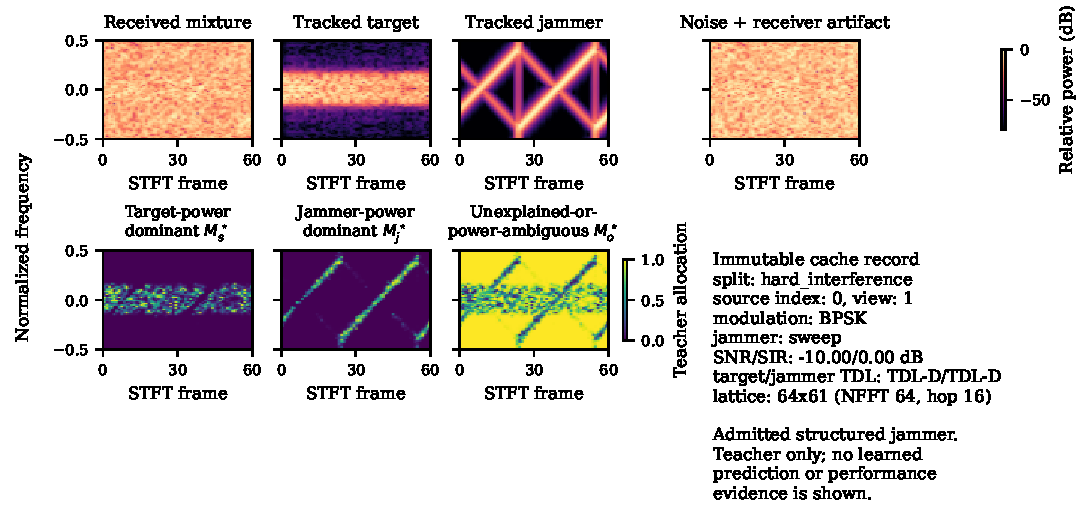
\includegraphics[width=0.85\textwidth]{figures/physical_teacher_example.pdf}
\caption{Training-only supervision for the compact spectral routes. The top
row shows the received mixture and simulator-tracked target, jammer, and
residual components; the bottom row shows the corresponding target-dominant,
jammer-dominant, and uncertainty masks from Eqs.~(5)--(6). Only the received
mixture is available at inference.}
\label{fig:teacher}
\end{figure*}

\subsection{Training Objective}
The total loss is
\begin{equation}
\begin{split}
\mathcal{L}&=\mathcal{L}_{\mathrm{mod}}+\alpha\mathcal{L}_{\mathrm{teacher}}
+\beta\mathcal{L}_{\mathrm{jammer}}+\gamma\mathcal{L}_{\mathrm{link}}\\
&\quad+\eta\mathcal{L}_{\mathrm{contrast}}+\theta\mathcal{L}_{\mathrm{orth}},
\end{split}
\end{equation}
where $\mathcal{L}_{\mathrm{mod}}$ is the modulation classification loss,
$\mathcal{L}_{\mathrm{teacher}}$ is a Jensen--Shannon \cite{lin1991js}
alignment between student and teacher masks, $\mathcal{L}_{\mathrm{jammer}}$ and $\mathcal{L}_{\mathrm{link}}$
constrain the jammer-family and link-quality auxiliary objectives,
$\mathcal{L}_{\mathrm{contrast}}$ is a supervised-contrastive loss
\cite{khosla2020supcon} over exact-source positives that encourages condition
invariance, $\mathcal{L}_{\mathrm{orth}}$ is a route-orthogonality regularizer,
and $\alpha,\beta,\gamma,\eta,\theta$ are
nonnegative weights. The exact-source contrastive loss is an auxiliary
training objective.

\subsection{Information Contract and Complexity}
At inference every model receives only the mixture; simulator-tracked target,
jammer, and SIR quantities are training-only or post-hoc audit variables.
\method\ uses \ParamsAFive\ parameters and \MacsAFive\ million reported MACs.

\subsection{Implementation Details}
\label{sec:impl}
Unless otherwise stated, all models share the same \mbox{source-disjoint} cache, data
budget, optimization budget, stopping rule, and validation-only selection
criterion; model-specific components follow each variant's predefined
configuration.

\emph{Input and front end.} One example is a complex baseband window of
\WindowSamples\ samples ($\WindowMicroseconds$ $\mu$s at \SampleRateMHz\ MHz,
\SamplesPerSymbol\ samples per symbol, root-raised-cosine roll-off
\RrcRolloff), power-normalized by the frozen receiver automatic gain control. The spectral
front end
applies a two-sided STFT with $N_{\mathrm{FFT}}=\NFft$, hop \HopLength, a
periodic Hann window of length \NFft, and no centering or zero padding, giving
a \StftBins$\times$\StftFrames\ time--frequency lattice at \StftBinHz\ kHz per
bin. The student and the fixed teacher share this lattice exactly.

\emph{Architecture width.} The sealed configuration uses \SpectralChannels\
spectral channels, embedding dimension \EmbeddingDim, environment dimension
\EnvironmentDim, and dropout \DropoutRate, for \ParamsAFive\ parameters. The
prospective capacity ladder widens only these three numbers: the M tier uses
(\CapacityMSpectral, \CapacityMEmbedding, $48$) and the L tier
(\CapacityLSpectral, \CapacityLEmbedding, $64$).

\emph{Optimization and model selection.} All fits use AdamW with an initial
learning rate of $\TrainLR$, weight decay $\TrainWeightDecay$, batch size
\TrainBatch, mixed precision, gradient-norm clipping at \GradClip, and a shared
\TrainEpochs-epoch budget. Auxiliary losses follow a fixed staged schedule,
after which the learning rate decays on a cosine to a floor of $0.05$ times
its initial value. The reported checkpoint is chosen solely by validation
modulation cross-entropy under a common eligibility window and
\TrainPatience-epoch early-stopping rule. No comparator received an
architecture-specific sweep, and validation data are never used for
evaluation.

\emph{Loss weights.} In~(7), $\alpha=\LossAlpha$, $\beta=\LossBeta$,
$\gamma=\LossGamma$, $\eta=\LossEta$, and $\theta=\LossOrtho$, with label
smoothing \LabelSmoothing\ and contrastive temperature \ContrastTemp. The
route-orthogonality regularizer is part of the A5 bundle but not isolated.

\emph{Seeds.} The sealed campaign uses \ProtocolSeedCount\ algorithm seeds
shared across all models, with seed-aligned initialization; matched-subset
displays use the first five. Schedules, seeds, teacher construction, and
cache provenance are recorded in the reproduction package.

\section{Experimental Design and Statistical Analysis}
\subsection{Source-Disjoint Simulation Campaign}
Macro-F1 is the primary score; it gives each modulation class equal weight,
including classes with fewer examples.
The fixed campaign contains \ProtocolModelCount\ model variants,
\ProtocolSeedCount\ algorithm seeds, \ProtocolFitCount\ fits,
\ProtocolSplitCount\ evaluation splits, and \ProtocolTrainSources\ training
source sequences. Target classes are BPSK, PI/2-BPSK, QPSK, 8PSK, 16QAM, 64QAM, 256QAM, GMSK,
CPFSK, and 4FSK, covering PSK, QAM, continuous-phase, and FSK families.
Structured jammer families span tone, multitone, chirp, sweep, partial-band,
pulse, comb, and out-of-taxonomy (cochannel and OFDM-like) modulated sources. TDL-A/C/D
profiles are seen during training, while TDL-B/E profiles support held-channel
evaluation. The evaluation grid spans \SnrGridCount\ SNR levels from
$\SnrGridLow$ to $\SnrGridHigh$ dB. SNR measures target strength relative to
receiver noise, whereas SIR measures target strength relative to the jammer;
more negative SIR therefore means stronger interference. The in-distribution split uses SIR levels
$-10$ to $10$ dB in $5$ dB steps, whereas the hard-interference split spans
SIR $\in\{-15,-10,-5,0\}$ dB, so SIR $=-15$ dB occurs only in the
hard-interference split and SIR $=+5$ and $+10$ dB only in the in-distribution
split. Each hard-interference SNR--SIR evaluation cell of
Fig.~\ref{fig:operating-map} contains 131--181 \mbox{source-disjoint} test windows
(mean 156; all ten classes, 5--26 per class), read from the frozen prediction
cache. The envelope aggregates of Section~V-D use a coarser partition of the
same predictions (216--279 \mbox{source-disjoint} windows per held cell, mean 250). The fit-domain division
(in-distribution plus hard-interference cells) is fixed in the exploratory
analysis protocol before any envelope is fitted. Jammer family, speed, channel, combined OOD, receiver stress, and
clean-retention splits share source identities across model comparisons. The
receiver-stress split (ADC quantization and per-emitter synchronization) is
retained in the artifact package but does not enter any sealed, envelope, or
reported selector claim.

\subsection{Comparator Fairness}
Table~\ref{tab:baselines} summarizes the comparators. All models are retrained
under the same \mbox{source-disjoint} protocol; ``IQFormer-inspired'' and
``MCLDNN'' denote architecture-faithful unified-retraining references, not
exact reproductions of every original training recipe. Comparator fairness is
enforced at the budget rather than at the tuning level: every model sees the
same training source count, the same epoch budget, the same early-stopping
patience and checkpoint criterion, and the same validation protocol. CSSL is
retained as a supervised adaptation reference;
its 8.63 million parameters but only 155.3 million MACs reflect aggressive
encoder downsampling and a large projection head, so parameter count alone is
a poor cost proxy for this comparator. Figures label this comparator
``IQFormer-insp.''; ``A5''
and ``\method'' denote the same sealed configuration, and ``CSSL'' abbreviates
the contrastive self-supervised learning reference of
\cite{du2025contrastive}, whose released code snapshot \cite{du2025csslcode} we
retrain under our protocol. Because this campaign retrains CSSL under the
common supervised budget without executing the released self-supervised
pretraining stage, it is reported as a supervised adaptation reference rather
than a reproduction of the full released recipe.

\begin{table}[t]
\centering
\caption{Comparator and Complexity Summary (Hard-Interference Setting).}
\label{tab:baselines}
\footnotesize
\setlength{\tabcolsep}{2.6pt}
\begin{tabular}{lcccc}
\toprule
Model & Domain & Params & MACs & Seeds\\
\midrule
A0 & spectral & \ParamsAZero & \MacsAZero\,M & 10\\
A5 / \method & spectral allocation & \ParamsAFive & \MacsAFive\,M & 10\\
sidecar & spectral + received I/Q & \SidecarParameters & \SidecarMacsTotal\,M & 10\\
MCLDNN & I/Q & \ParamsMCLDNN & \MacsMCLDNN\,M & 10\\
IQFormer-inspired & multimodal I/Q & \ParamsIQFormer & \MacsIQFormer\,M & 10\\
CSSL & I/Q (adaptation) & \ParamsCSSL & \MacsCSSL\,M & 10\\
\bottomrule
\end{tabular}
\end{table}

% E1 numbers from artifacts/rml2016_10a_fidelity_v3/metrics.csv (three seeds,
% 17/29/43; per-stratum 80/20 then 75/25 train_test_split(random_state=233) =
% 600/200/200; all-SNR test accuracy over the 20-SNR grid). Published
% reference: official IQFormer benchmark result table testA.xlsx
% (paper_data_layer/outputs/e1_reference.json; MCLDNN 62.05%, IQFormer 64.19%).
As a public-benchmark comparator-fidelity check, the MCLDNN and IQFormer
implementations were additionally evaluated on the public RML2016.10a benchmark
\cite{oshea2016cnn} under the official IQFormer-release benchmark protocol
\cite{shao2025iqformercode}: the 11-class set, the
full $-20$ to $18$ dB SNR grid, per-stratum $600/200/200$ splits seeded at
$233$, no augmentation or input-length change. Over three algorithm seeds,
all-SNR test accuracy is $58.55\%$ for MCLDNN (seed range
$58.1$--$59.4\%$) and $65.23\%$ for IQFormer-inspired ($64.8$--$65.8\%$;
seed ranges, not confidence intervals); the reference-release values,
averaged over the same twenty SNR bins, are $62.05\%$ and $64.19\%$.
IQFormer-inspired closely matches the
reference-release all-SNR accuracy ($+1.04$~pp), whereas MCLDNN remains
moderately lower ($-3.50$~pp) while staying in the same
broad all-SNR range. Per-SNR deviations of up to about $8$~pp remain, so E1
speaks only to range-level comparator-implementation fidelity.

\subsection{Baseline Configuration Contrast}
The original confirmatory family contains three hard-interference contrasts:
the complete
configuration versus A0, the margin teacher versus a proportional-power
teacher, and the tri-route model versus a dual-route control. A5 differs from
A0 in allocation, teacher, auxiliary objectives, residual bypass, and capacity
(about $4.7\times$ parameters), so A5--A0 is a whole-configuration
effect.

\subsection{Evidence Scope and Independent Validation}
The three configuration contrasts were fixed before the campaign analysis.
The SNR--SIR map, overlap envelope, fusion, and capacity studies are
exploratory analyses of the campaign predictions, including the post-hoc
$-15$-dB SIR stratification. They describe where the ranking changes but do not
establish that the same boundary will hold in a new regime.

That transport question is evaluated on an independently generated
severe-held set. The transfer analysis was specified before inference on that
set. The sidecar analysis was specified after the transfer result but before
sidecar evaluation, and the attribution controls were fixed before their
respective executions. This sequence separates the original configuration
contrast, campaign diagnosis, independent transport test, and subsequent
repair intervention. The Supplement records the detailed execution timeline
and reproducibility provenance.

\subsection{Statistical Procedures}
The original confirmatory family uses a joint non-studentized max-absolute-deviation
hierarchical paired bootstrap with \ProtocolBootstrapDraws\ draws, resampling
class-stratified source clusters while keeping algorithm seeds as fixed
blocks, so pairing is preserved at the source level. The design resolution of
\DesignResolution\ \pp\ is the simultaneous minimum detectable effect at 80\%
power under this joint interval, an exploratory calibration. Because seeds are fixed blocks, the reported
intervals are conditional on the realized seed set; a seed-randomization
variant resampling the ten realized seeds with replacement keeps the A5--A0
contrast positive (95\% percentile interval
$[\SeedRandomEffectLow,\SeedRandomEffectHigh]$ \pp) while the teacher-form and
route-count contrasts span zero
($[\SeedRandomTeacherLow,\SeedRandomTeacherHigh]$ and
$[\SeedRandomRouteLow,\SeedRandomRouteHigh]$ \pp). In the campaign's severe row, all
\SevereGainIqformerPositiveSeeds\ seeds share the same sign; the sign-flip
permutation probability \SevereGainIqformerSignFlipP\ is a permutation test
over the source-paired samples. The SIR $=-15$ dB aggregate is computed from
source-paired predictions pooled across the eight SNR conditions before
macro-F1 aggregation; it is therefore not the arithmetic mean of the eight
displayed cell-level differences in Fig.~\ref{fig:operating-map}. The
severe-held levels and repair contrasts of Section~V-G instead average
per-seed macro-F1 values with equally weighted regimes (the seed-wise paired
convention); the two conventions are never mixed within a single reported
contrast.

\section{Results}
\subsection{Compact Baseline Configuration}
Table~\ref{tab:confirmatory} reports the original confirmatory family. The complete
configuration improves over its shared A0 backbone by \MethodEffectDiff\ \pp,
with a simultaneous interval of
$[\MethodEffectSimLow,\MethodEffectSimHigh]$ \pp, about 3.5 times
the design resolution of \DesignResolution\ \pp. The teacher-form and
route-count interventions do not clear zero individually; under the same joint
interval their simultaneous upper bounds are $\TeacherFormSimHigh$ and
$\TriRouteSimHigh$ \pp, respectively.
Thus the configuration-level effect is resolved but cannot be assigned to
either isolated component at this resolution. Because the prespecified joint
criterion required all three contrasts to exclude zero, the joint criterion
was not satisfied. The A5--A0 contrast nevertheless remains positive under the
simultaneous family-wise interval. At the same
parameter tier, the residual-free A7 variant is nominally above A5 by
\ASevenVsAFiveHardDiff\ \pp\ in the marginal hard-interference aggregate
(Supplement Table~IV); treating the ten realized seeds as a random effect
gives a 95\% percentile interval of
$[\ASevenVsAFiveSeedLow,\ASevenVsAFiveSeedHigh]$ \pp, so the difference is not
resolved at this design's power; we attribute the compact frontier
position to the VIMD family at this budget as a whole.

\begin{table}[t]
\centering
\caption{Original Confirmatory Hard-Interference Family. Differences Are
Candidate Minus Reference in Macro-F1 Percentage Points.}
\label{tab:confirmatory}
\footnotesize
\setlength{\tabcolsep}{3.2pt}
\begin{tabular}{lrrr}
\toprule
Contrast & Diff. & Sim. low & Sim. high\\
\midrule
Full configuration vs A0 & $\MethodEffectDiff$ & $\MethodEffectSimLow$ & $\MethodEffectSimHigh$\\
Margin vs proportional teacher & $\TeacherFormDiff$ & $\TeacherFormSimLow$ & $\TeacherFormSimHigh$\\
Tri-route vs dual-route & $\TriRouteDiff$ & $\TriRouteSimLow$ & $\TriRouteSimHigh$\\
\bottomrule
\end{tabular}
\end{table}

\subsection{Condition-Dependent Ranking within the Campaign}
Marginal hard-interference macro-F1 is \AbsAFiveHard\ for A5,
\AbsMCLDNNHard\ for MCLDNN, and \AbsIQFormerHard\ for IQFormer-inspired;
the averages favor the larger models. Figure~\ref{fig:operating-map} shows why no
single campaign-level ranking is adequate: the sign changes with SNR and SIR,
including a severe-row reversal. Section~V-C tests whether this campaign
structure transfers to independently generated severe regimes.

\begin{figure*}[t]
\centering

\includegraphics[width=0.95\textwidth]{../paper_figures/outputs_v46/fig2_rank_instability.pdf}
\caption{Campaign-internal post-hoc rank instability over all hard-
interference SNR--SIR cells. Each entry is A5 minus the named I/Q reference in
macro-F1 percentage points. Blue cells favor A5 and orange cells favor the
reference; color and printed values encode the same sign. A star marks a
positive unadjusted paired lower interval; Holm-surviving cells are reported
in the text.}
\label{fig:operating-map}
\end{figure*}

At SIR $=-15$ dB, in a post-hoc analysis, A5 gains \SevereGainMcldnn\ \pp\ over
MCLDNN ($[\SevereGainMcldnnLow,\SevereGainMcldnnHigh]$) and
\SevereGainIqformer\ \pp\ over IQFormer-inspired
($[\SevereGainIqformerLow,\SevereGainIqformerHigh]$); these two headline
intervals are marginal stratified-bootstrap intervals and are not
multiplicity-adjusted. All
\SevereGainIqformerPositiveSeeds\ seeds have the same sign, and the sign-flip
permutation probability is \SevereGainIqformerSignFlipP. Of
\SevereCellsInspected\ inspected cells, \SevereCellsSurvivingHolm\ survive Holm
correction; all are on the severe SIR row. Together, these checks show that the
severe-row reversal is internally consistent across seeds and cells, while its
interpretation remains campaign-specific. Section~V-C evaluates this
interpretation on independently generated severe-held data, where the favorable
ordering does not persist.
The reversal against MCLDNN is not explained by a binding training cap:
MCLDNN early-stops in all ten seeds with best epochs well inside the shared
budget (median 13, range 11--16; Supplement Table~VIII).

\subsection{Independent Severe-Regime Transport Boundary}
An independently generated severe-held set tests whether the campaign's
$-15$-dB ordering survives broader regime changes. SIR remains fixed at
$-15$~dB: R1 combines held jammer families with 180-km/h mobility over training
channels, whereas R2 combines held channels with the same jammer families at
250~km/h. Relative to the campaign corner, R1 changes jammer family and speed;
R2 changes jammer family, speed, and channel. Each regime spans eight SNRs and
\SevereHeldSourcesPerRegime\ source-disjoint examples
(\SevereHeldSourcesTotal\ total), and all evaluated checkpoints remain fixed.

The campaign ordering does not persist. Under the seed-wise convention,
IQFormer-inspired and MCLDNN lead A5 by \SevereReferenceLeadIqformer\ and
\SevereReferenceLeadMcldnn\ \pp, respectively; the corresponding
window-pooled leads are \SevereTransferLeadIqformer\ and
\SevereTransferLeadMcldnn\ \pp. The campaign-derived overlap--SIR diagnostic
surface of Section~V-D also loses transport skill: its sign accuracy on the
severe-held cells falls to \SevereTransferSignAccIqformer\ against
IQFormer-inspired and \SevereTransferSignAccMcldnn\ against MCLDNN, while
SIR-only or constant predictors outperform the full surface. Thus, the
campaign's favorable compact-model corner and its
diagnostic boundary do not define a transferable severe-regime ordering.

The held jammer families clarify the remaining performance levels. Under
OFDM-like interference every evaluated model is near the floor
(\SevereHeldFamilyOfdmAFive\% for A5), whereas the pulse family remains
learnable (\SevereHeldFamilyPulseAFive\% for A5 and
\SevereHeldFamilyPulseMcldnn\% for MCLDNN). This difference also means that
jammer-family difficulty and out-of-domainness are confounded in the joint
transfer result. Per-family and per-regime levels are provided in the
Supplement.

\subsection{Campaign Diagnostic and Its Transport Limit}
The campaign-internal rank instability motivates a low-dimensional diagnostic
surface that summarizes how gain varies with target-support jammer overlap and
SIR. For reference $b$, we fit
\begin{equation}
\Delta_b=\beta_{0,b}+\beta_{1,b}o+\beta_{2,b}\,\mathrm{SIR},
\label{eq:envelope}
\end{equation}
where $\Delta_b$ is A5 minus the reference macro-F1 and $o$ is the
\emph{target-support jammer overlap}. We avoid the more common ``spectral
occupancy'' because $o$ is not an occupied-bin or occupied-bandwidth fraction.
The covariate is defined from the simulator-tracked target and jammer
components rather than from the mixture. For each window we compute the STFT
power of the tracked target and of the tracked jammer separately, order the
time--frequency cells by descending target power, and take the target's
99\%-energy support $\mathcal{S}$ as the smallest set of cells whose cumulative
target power reaches 99\% of the total. The overlap is then the fraction of the
jammer's total STFT power that falls inside $\mathcal{S}$:
\begin{equation}
o=\frac{\sum_{(f,t)\in\mathcal{S}}P_j(f,t)}{\sum_{(f,t)}P_j(f,t)}.
\label{eq:overlap}
\end{equation}
Thus $o=0.8$ means that 80\% of the jammer's energy lies within the target's
dominant support, not that the jammer fills 80\% of the plane. The cell-level
covariate is the mean of $o$ over the windows of that cell.

The overlap is computed from simulator-tracked components on a fixed analysis
lattice before model training; it is neither a receiver input nor a quantity
available to an uncooperative receiver. The fit uses \EnvelopeFitCells\ cells
from the in-distribution and hard-interference splits, and evaluation uses
\EnvelopeHoldoutCells\ cells from unseen-jammer, unseen-speed, held-channel,
and combined-OOD splits. Each cell retains all ten classes and at least 150
source-disjoint windows. Complete cell construction and sensitivity checks are
provided in the Supplement. Equation~\eqref{eq:envelope} is interpreted as a
descriptive summary rather than a causal model.

Against IQFormer-inspired, the surface reduces held-cell RMSE from
\EnvelopeConstantRmseIQ\ to \EnvelopeIqformerHoldoutRmse\ \pp\
($R^2_{\mathrm{skill}}=\EnvelopeSkillRTwoIQ$); against MCLDNN the corresponding
values are \EnvelopeConstantRmseMC\ and \EnvelopeMcldnnHoldoutRmse\ \pp\
($R^2_{\mathrm{skill}}=\EnvelopeSkillRTwoMC$). This pooled skill is
regime-dependent, and paired tests do not resolve an incremental overlap effect
beyond SIR. More importantly, leave-$-15$-dB-out tests and the independent
severe-held evaluation fail to support the full surface over simpler SIR-only
or constant predictors. Figure~\ref{fig:envelope} therefore visualizes a useful
campaign summary, not a transferable switching rule.

\begin{figure*}[t]
\centering

\includegraphics[width=0.75\textwidth]{../paper_figures/outputs_v46/fig3_campaign_diagnostic_envelope.pdf}
\caption{Campaign-diagnostic overlap--SIR envelope against IQFormer-inspired.
Panel~(a) uses the target-support jammer overlap, not occupied bandwidth:
filled markers are the \EnvelopeFitCells\ fit cells and open markers the
\EnvelopeHoldoutCells\ held cells. Panel~(b) compares predicted and observed
held-cell gain: RMSE \EnvelopeIqformerHoldoutRmse\ \pp\ versus
\EnvelopeConstantRmseIQ\ \pp\ for the frozen fit-domain constant
($R^2_{\mathrm{skill}}=\EnvelopeSkillRTwoIQ$). The surface summarizes
campaign-internal rank variation but does not transport to the independent
severe-held regimes of Section~V-C.}
\label{fig:envelope}
\end{figure*}

The fitted break-even references and the unexpected positive overlap direction
remain simulator-domain observations. Because the directional expectation was
rejected and overlap is not directly observable at the receiver, these
quantities are retained only as diagnostic evidence.

\subsection{Complementarity and Cost Motivation}
On the campaign hard-interference split, late probability fusion improves over
the stronger constituent by \FusionIqformerGain\ \pp\ with IQFormer-inspired
and \FusionMcldnnGain\ \pp\ with MCLDNN. Same-model two-seed ensembles improve
by \FusionIqformerControl\ and \FusionMcldnnControl\ \pp. Computed from the
unrounded values, the corresponding excess cross-model fusion gains are
\FusionIqformerExcess\ and \FusionMcldnnExcess\ \pp.
This difference is consistent with complementarity beyond ordinary same-model
ensembling. The diagnostic requires concurrent execution of both models and
was not evaluated as the severe-held repair mechanism.

Table~\ref{tab:baselines} gives the corresponding parameter and MAC budgets;
compactness is stated as a parameter and MACs property.

\subsection{Diagnosing the Representation Limitation}
The cross-regime severe degradation makes representation robustness central
to interpretation. The earlier clean-condition diagnosis
independently tests whether the compact spectral representation discards
information that becomes important under distribution shift.
The clean-retention split contains all ten modulations, but the two training
views expose jammer-free windows for only \TrainClassesWithCleanWindows\
classes (PI/2-BPSK, 8PSK, 256QAM, and CPFSK); the remaining
\TrainClassesWithoutCleanWindows\ classes (BPSK, QPSK, 16QAM, 64QAM, GMSK, and
4FSK) are a condition-transfer test. The four covered classes are marked
without a star in Fig.~\ref{fig:transfer}, where a star denotes a class whose
jammer-free condition was not seen during training. Transfer failure occurs
in $27/27$ uncovered compact-spectral class--model cells
(\TransferFailShareCompact\%) versus $1/9$ I/Q-reference cells
(\TransferFailShareHighCapacity\%). The
clean-retention gate did not pass. Figure~\ref{fig:transfer} localizes the
failure at the class level.

\begin{figure}[!b]
\centering
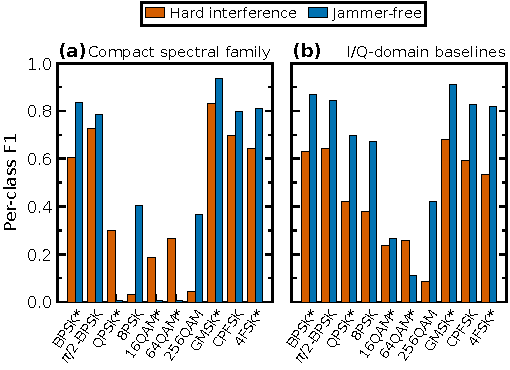
\includegraphics[width=\columnwidth]{../paper_figures/outputs_origin/fig4_clean_condition_transfer.pdf}
\caption{Clean condition-transfer taxonomy. Bars show family-mean per-class
F1 under hard interference (orange) and jammer-free evaluation (blue)
for the compact spectral family and I/Q-domain baselines. A star marks a class
whose jammer-free condition was absent from training; it is not a significance
marker.}
\label{fig:transfer}
\end{figure}

We then followed a prospective decision chain.
Frozen-checkpoint linear and MLP probes used a correctly reconstructed
jammer-free counterfactual and \mbox{source-disjoint} clean cross-validation; probe
performance is the unweighted mean F1 over QPSK, 16QAM, and 64QAM (chance
$\approx0.1$ on ten classes). The predefined decision rule declares a representation
\emph{information-present, head-limited} when this mean exceeds
\ProbeThreshold\ and \emph{representation-limited} otherwise, requiring
\emph{all} design--seed cells to exceed the threshold. For A5,
five of the six design--seed cells (three algorithm
seeds $\times$ the reconstructed jammer-free counterfactual and clean
cross-validation probes) lie below the \ProbeThreshold\ threshold; the sole
cell above it is borderline at $0.256$. Because the decision changes under a
$0.20$ threshold, we treat the probe result as directional evidence for
representation limitation rather than as a threshold-robust classification of
mechanism.
The strong I/Q baselines exceed the threshold in
\ProbeStrongAboveThreshold\ of \ProbeStrongCells\ cells. The evidence
therefore leans toward missing constellation information in the compact
spectral representation rather than a classification head that fails to use
available information.

Adding clean windows for every class tests the simpler coverage explanation.
It changes clean macro-F1 by only $\CoverageCleanDiff$\ \pp\
($[\CoverageCleanLow,\CoverageCleanHigh]$) and hard macro-F1 by
$\CoverageHardDiff$\ \pp\ ($[\CoverageHardLow,\CoverageHardHigh]$). Coverage
alone is therefore insufficient. A predefined negative control gates the
modulation route using predicted interference presence. Relative to A5, it
changes clean macro-F1 by $\PresenceGateCleanVsAFiveDiff$\ \pp\
($[\PresenceGateCleanVsAFiveLow,\PresenceGateCleanVsAFiveHigh]$) and hard
macro-F1 by $\PresenceGateHardVsAFiveDiff$\ \pp\
($[\PresenceGateHardVsAFiveLow,\PresenceGateHardVsAFiveHigh]$). The learned
gate averages \PresenceGateCleanMean\% on clean windows and
\PresenceGateHardMean\% under hard interference, saturating near the modulated
route; this arm serves as a negative control.

\subsection{Low-Cost I/Q Repair and Attribution}
Widening the spectral model without changing its representation domain first
separates capacity from representation. The widest spectral tier remains below
IQFormer-inspired on the campaign hard split (L$-$IQFormer-inspired:
$\CapacityLHardVsIqformerDiff$ percentage points
[$\CapacityLHardVsIqformerLow,\CapacityLHardVsIqformerHigh$]) and on clean
retention ($\CapacityLCleanVsIqformerDiff$
[$\CapacityLCleanVsIqformerLow,\CapacityLCleanVsIqformerHigh$] percentage
points). At SIR $=-15$~dB it gains only $+\CapacityLSevereVsSDiff$ \pp\
($[\CapacityLSevereVsSLow,\CapacityLSevereVsSHigh]$) over the sealed tier.
Tested spectral width scaling alone therefore does not remove the
representation limitation.

\begin{table*}[t]
\centering
\caption{Transport, Repair, and Attribution Controls. Positive contrasts favor
the row model; where reported, confidence intervals are seed-wise paired 95\%
intervals. Lesion rows measure inference-time sensitivity of the jointly
trained sidecar. Panel (c) reports a five-seed variant trained on the original
campaign partitions with its I/Q input permanently zeroed; severe-held data
remain evaluation-only.}
\label{tab:severe_summary}
\footnotesize
\setlength{\tabcolsep}{6pt}
\textbf{(a) Full ten-seed severe-held evaluation}\\[2pt]
\begin{tabular*}{0.92\textwidth}{@{\extracolsep{\fill}}lccc@{}}
\toprule
Model or intervention & Macro-F1 (\%) & Reference & Contrast\\
\midrule
A5 spectral baseline & \SevereRepairLevelAFive & --- & reference level\\
IQFormer-inspired & \SevereRepairLevelIqformer & A5 & $+\SevereReferenceLeadIqformer$ \pp\\
MCLDNN & \SevereRepairLevelMcldnn & A5 & $+\SevereReferenceLeadMcldnn$ \pp\\
Received-I/Q sidecar & \textbf{\SevereRepairLevelSidecar} & A5 & $+\SevereRepairDiff$ \pp\ ($[\SevereRepairCiLow,\SevereRepairCiHigh]$)\\
Sidecar, I/Q zeroed & \SevereControlLevelIqZero & full sidecar & $-\SevereControlIqZeroLoss$ \pp\\
Sidecar, I/Q shuffled & \SevereControlLevelIqShuffle & full sidecar & $-\SevereControlIqShuffleLoss$ \pp\\
Sidecar, side head removed & \SevereControlLevelNoSideHead & full sidecar & $-\SevereControlNoSideHeadLoss$ \pp\ ($\SevereControlDiffNoSideHead$ \pp\ vs.\ A5)\\
\bottomrule
\end{tabular*}

\vspace{4pt}
\textbf{(b) Matched five-seed capacity control}\\[2pt]
\begin{tabular*}{0.92\textwidth}{@{\extracolsep{\fill}}lcccc@{}}
\toprule
Measure & A5 & Width M & Width L & I/Q sidecar \\
\midrule
Macro-F1 (\%) & \SevereControlMatchedLevelAFive & \SevereControlLevelCapM & \SevereControlLevelCapL & \textbf{\SevereControlMatchedLevelSidecar} \\
MACs (M) & \MacsAFive & \CapacityMMacs & \CapacityLMacs & \SidecarMacsTotal \\
Seeds & 5 & 5 & 5 & 5 \\
\bottomrule
\end{tabular*}

\vspace{4pt}
\textbf{(c) Retrained attribution ablation}\\[2pt]
\begin{tabular*}{0.92\textwidth}{@{\extracolsep{\fill}}lcccc@{}}
\toprule
Condition & Macro-F1 (\%) & Reference & Contrast & Seeds\\
\midrule
Sidecar retrained, I/Q permanently zeroed & \RetrainedIqzeroPooledLevel & A5 & $\RetrainedIqzeroVsAFiveDiff$ \pp\ ($[\RetrainedIqzeroVsAFiveCiLow,\RetrainedIqzeroVsAFiveCiHigh]$) & 5\\
Full sidecar (matched seeds) & \textbf{\RetrainedFullPooledLevel} & A5 & $+\RetrainedFullVsAFiveDiff$ \pp\ ($[\RetrainedFullVsAFiveCiLow,\RetrainedFullVsAFiveCiHigh]$) & 5\\
\bottomrule
\end{tabular*}
\end{table*}

The sidecar pools mean, standard deviation, and maximum statistics from a
two-channel depthwise-separable received-I/Q branch, fuses its 24-dimensional
embedding residually with the spectral path, and adds a side head. It uses only
the received mixture and adds about 3\% compute over A5. On the original
campaign, the same configuration gains $\SidecarCleanVsAFiveDiff$~\pp\ on
clean retention and $\SidecarHardVsAFiveDiff$~\pp\ on the hard split relative
to A5.

On the same frozen severe-held benchmark that exposed the transport boundary,
the prospectively specified sidecar raises seed-mean
pooled macro-F1 from \SevereRepairLevelAFive\% to
\SevereRepairLevelSidecar\%, a paired gain of \SevereRepairDiff\ \pp\
($[\SevereRepairCiLow,\SevereRepairCiHigh]$). Repair is positive in all
\SevereRepairPositiveSeeds\ seeds and all \SevereRepairPositiveSnrStrata\ SNR
strata. Absolute macro-F1 remains low for every model at this extreme operating
point, so the gain is interpreted as robustness repair. Coincidentally, the
campaign hard-split sidecar gain is also \SevereRepairDiff\ \pp, but it is a
distinct ten-seed measurement with interval
[$\SidecarHardVsAFiveLow,\SidecarHardVsAFiveHigh$] \pp.
Because this domain had already been characterized by the preceding transfer
test, the sidecar experiment evaluates a prospectively specified intervention
on a known held domain rather than an independent replication of repair
transport.

The controls in Table~\ref{tab:severe_summary} separate tested
spectral width scaling from received-I/Q information and the added fusion
head. On the matched five-seed severe-held subset, Width L gains only
$+\SevereControlDiffCapL$ \pp\ over A5 at \CapacityLMacs\ M MACs, whereas the
sidecar gains $+\RetrainedFullVsAFiveDiff$ \pp\
($[\RetrainedFullVsAFiveCiLow,\RetrainedFullVsAFiveCiHigh]$) at
\SidecarMacsTotal\ M MACs. Thus, the larger repair has substantially lower
incremental compute. The L tier's \CapacityLMacs\ M MACs are already within the
range of the large I/Q comparators (\MacsIQFormer\ M and \MacsMCLDNN\ M), so
the width ladder does not retain the compute advantage that motivates the
compact receiver. The remaining controls are
inference-time lesions of the jointly trained sidecar; each lesion removes
$\SevereControlIqShuffleRepairRatio$--$\SevereControlNoSideHeadRepairRatio$
times the magnitude of the repair effect, and the lesioned variants fall
below the unmodified A5 baseline. They establish inference-time dependence
on received-I/Q input but cannot quantify the branch's information
contribution. The follow-up retrained the same architecture on the original
campaign training and validation partitions with the I/Q input permanently
zeroed (five matched seeds and the same recipe); the severe-held set remained
evaluation-only. The zeroed variant gains
$\RetrainedIqzeroVsAFiveDiff$~\pp\ versus A5
($[\RetrainedIqzeroVsAFiveCiLow,\RetrainedIqzeroVsAFiveCiHigh]$), while the
matched full sidecar shows a gain of $\RetrainedFullVsAFiveDiff$~\pp\
($[\RetrainedFullVsAFiveCiLow,\RetrainedFullVsAFiveCiHigh]$). The zeroed variant
also remains at the A5 level on the campaign hard split, arguing against failed
optimization as the explanation. Thus, within the tested architecture and simulation
domain, the repair depends on informative received-I/Q input rather than on
the added capacity and fusion structure alone.

\section{Discussion}
\subsection{Implications for AMC Evaluation}
The experiments show that model ranking is condition- and regime-dependent.
Marginal scores favor the I/Q references, the campaign contains a
severe-condition reversal, and the independent severe-held regimes reverse
that ordering again. The appropriate object of comparison is therefore the
condition-dependent ranking, not a single global leaderboard.

This distinction changes the role of a compact-model gain. A favorable cell or
stratum identifies where a representation is competitive inside the tested
campaign; it does not establish that the same ordering will survive a joint
change in jammer family, mobility, and channel. Reporting both marginal and
condition-resolved rankings is therefore necessary when a learned receiver is
selected for a variable operating environment.

\subsection{Why the Campaign Diagnostic Does Not Transport}
Equation~\eqref{eq:envelope} has skill over 80 held cells inside the frozen
campaign, but that skill is heterogeneous by regime. The incremental overlap
effect beyond SIR is not separately resolved, and leave-$-15$-dB-out behavior
depends on the reference. Gain also increases rather than decreases with
overlap inside the campaign, opposite to the predefined directional
expectation. The surface is therefore most useful as a descriptive diagnostic.
Its overlap variable additionally requires
simulator-tracked target and jammer components and is not directly observable
at an uncooperative receiver.

The independently generated severe-held evaluation tests the campaign-internal
severe ranking under new jammer, mobility, and channel combinations. The
favorable ordering does not persist, defining a clear cross-regime transport
boundary. This result also shows why the in-campaign break-even references
should be treated as descriptive diagnostics rather than cross-regime
switching thresholds.

\subsection{Representation Repair and Receiver Design}
The severe-held controls expose a compute--representation asymmetry within the
tested architecture and regimes: substantial spectral widening does not
reproduce the repair, whereas a small received-I/Q path produces a much larger
gain under the reported MAC budget. Inference-time lesions show dependence
on the I/Q path, and the retrained zeroed-I/Q control shows that added capacity
and fusion structure without informative I/Q input do not reproduce the gain.
Within the tested architecture, these results identify received-I/Q
information as the factor enabling the repair. This identifies a mechanism-level
effect within the tested simulation setting; deployment performance remains to
be established.

At $f_c=\CarrierGHz$ GHz and the held-speed conditions, the channel can evolve
materially within the \WindowMicroseconds-$\mu$s decision window: the nominal
coherence time at \HeldSpeeds\ km/h is about $42\%$ and $30\%$ of the window,
increasing intra-window nonstationarity. Representation robustness is
therefore a receiver-design issue as well as a classifier-ranking issue. More
generally, the results caution against fixing a learned receiver architecture
or switching rule solely from one campaign's marginal leaderboard or condition
surface. For compute-constrained learned receivers, the practical lesson is to
test ranking stability across operating regimes and preserve a low-cost
complementary signal path when a compact representation is vulnerable to
shift.

\section{Limitations}
The study has several limitations. First, all results are based on
\mbox{source-disjoint} TR~38.901 TDL-profile simulations and do not
constitute over-the-air or MAC-/network-layer V2X validation. Second, the
confirmatory family resolves only the A5--A0 whole-configuration contrast; the
isolated teacher-form and route-count effects remain unresolved.
Third, the severe-held regimes change jammer family together with mobility,
and R2 also changes channel profile. The transfer result therefore bounds
joint transport and does not identify a single causal shift factor. Fourth,
IQFormer-inspired and CSSL reach the shared \TrainEpochs-epoch limit in all
seeds, so their comparisons retain a budget-sufficiency caveat; MCLDNN
early-stops in all seeds and is not subject to the same immediate cap. Fifth,
the overlap covariate requires simulator-tracked target and jammer components
that are unavailable at an uncooperative receiver. In addition, absolute
macro-F1 remains low in the extreme severe-held regime. The RML2016.10a check
addresses comparator-implementation fidelity rather than validation of the
proposed representation.
RML2016.10a does not expose the separately tracked post-channel target, jammer,
and residual components required by the training-only teacher, so it cannot
instantiate the full A5 training recipe.

\subsection*{Reproducibility}
The artifact package preserves the source data, cache identities, checkpoints,
analysis definitions, figure-source CSVs, per-seed aggregates, configurations,
and provenance associated with each evidence stage. Each manuscript macro
stores its source path, row selector, evidence class, precision, and source
SHA-256. Together, these records support direct reproduction of the reported
analyses; the resolved package will be released upon acceptance.

\section{Conclusion}
A single marginal AMC score is insufficient when the preferred signal
representation changes across interference and mobility regimes. The reported
campaign reveals such a rank reversal, while independent severe-held
evaluation shows that neither the favorable compact-model corner nor its
overlap--SIR diagnostic transfers uniformly to new regime combinations. A
lightweight received-I/Q sidecar recovers \SevereRepairDiff\ \pp\ on that
benchmark at about 3\% additional MACs. Spectral widening does not reproduce
the gain, and a retrained zeroed-I/Q variant returns to the spectral baseline,
supporting informative I/Q input as the enabling factor within the tested
architecture. Because absolute performance remains low and all evidence is
simulation-based, the result is a bounded robustness recovery. The broader
receiver-design implication is to test ranking stability explicitly and retain
a low-cost complementary signal path when compact representations are exposed
to regime shift.

\section*{Acknowledgment}
The authors used AI tools solely for English-language editing and figure-style
assistance. The authors verified all technical content, mathematical
derivations, data, code, statistical analyses, figure data and renderings,
interpretations, and conclusions, and take full responsibility for the work.

\IEEEtriggeratref{24}
\bibliographystyle{IEEEtran}
\bibliography{references}

\end{document}
